%% 由 build/emit_tex.py 生成（生成物，勿手改）；定制请放 user_style.tex / user_meta.yaml
\chapter{Scipy及其基本使用}\label{scipyux53caux5176ux57faux672cux4f7fux7528}

\section{01
微积分工具包：数值积分与微分方程数值解}\label{ux5faeux79efux5206ux5de5ux5177ux5305ux6570ux503cux79efux5206ux4e0eux5faeux5206ux65b9ux7a0bux6570ux503cux89e3}

\begin{quote}
本节对应原版 3.1 的内容，并增补学习目标、常见误区、思考题与延伸阅读。
所有代码均在 SciPy 1.15.2 / NumPy 2.1.2 环境实际运行验证。
配套图：\texttt{figures/03-scipy/ode\_solution.png}（由
\texttt{build/make\_chap3\_figures.py} 生成）。
\end{quote}

\subsection{本节目标}\label{ux672cux8282ux76eeux6807-6}

\begin{itemize}
\tightlist
\item
  会用手工梯形公式近似定积分，理解``分割越细越精确''的收敛思想；
\item
  会用 \texttt{scipy.integrate.quad} 求一维定积分，用
  \texttt{dblquad}/\texttt{nquad} 求多重积分；
\item
  会用 \texttt{trapezoid} 对离散数据（实验数据/数值解）做数值积分；
\item
  会用 \texttt{odeint}/\texttt{solve\_ivp}
  求解一阶、高阶及常微分方程组；
\item
  了解 \texttt{solve\_bvp} 用于边值问题。
\end{itemize}

\subsection{先修}\label{ux5148ux4fee-6}

\begin{itemize}
\tightlist
\item
  第 1 章 NumPy：\texttt{np.linspace}、\texttt{np.arange}、数组切片；
\item
  第 2 章 SymPy：知道解析积分与数值积分的区别（可先跳过）。
\end{itemize}

\subsection{官方文档 /
参考入口}\label{ux5b98ux65b9ux6587ux6863-ux53c2ux8003ux5165ux53e3}

\begin{itemize}
\tightlist
\item
  SciPy
  积分模块总览：https://docs.scipy.org/doc/scipy/reference/integrate.html
\item
  \texttt{quad}：https://docs.scipy.org/doc/scipy/reference/generated/scipy.integrate.quad.html
\item
  \texttt{solve\_ivp}：https://docs.scipy.org/doc/scipy/reference/generated/scipy.integrate.solve\_ivp.html
\end{itemize}

\begin{center}\rule{0.5\linewidth}{0.5pt}\end{center}

\subsection{1.1
为什么需要数值积分}\label{ux4e3aux4ec0ux4e48ux9700ux8981ux6570ux503cux79efux5206}

很多函数的原函数无法写成初等函数（例如
\(e^{-x^2}\)、\(\sin(x^2)\)），或者我们只有离散的实验采样点。此时只能用数值方法求定积分。

\subsubsection{1.1.1
梯形法：从手工到库函数}\label{ux68afux5f62ux6cd5ux4eceux624bux5de5ux5230ux5e93ux51fdux6570}

把 \([a,b]\) 等分成 \(n\) 段，每段用梯形近似曲线下面积：

\[\int_a^b f(x)\,dx \approx \sum_{i=0}^{n-1}\frac{f(x_i)+f(x_{i+1})}{2}\cdot h,\quad h=\frac{b-a}{n}\]

下面用 Python 实现 \(\int_0^1 x^2 dx\)，理论值 \(\frac{1}{3}\)。

\begin{Shaded}
\begin{Highlighting}[]
\KeywordTok{def}\NormalTok{ trapezoidal\_rule(f, a, b, n):}
\NormalTok{    h }\OperatorTok{=}\NormalTok{ (b }\OperatorTok{{-}}\NormalTok{ a) }\OperatorTok{/}\NormalTok{ n}
\NormalTok{    s }\OperatorTok{=} \FloatTok{0.5} \OperatorTok{*}\NormalTok{ (f(a) }\OperatorTok{+}\NormalTok{ f(b))}
    \ControlFlowTok{for}\NormalTok{ i }\KeywordTok{in} \BuiltInTok{range}\NormalTok{(}\DecValTok{1}\NormalTok{, n):}
\NormalTok{        s }\OperatorTok{+=}\NormalTok{ f(a }\OperatorTok{+}\NormalTok{ i }\OperatorTok{*}\NormalTok{ h)}
    \ControlFlowTok{return}\NormalTok{ s }\OperatorTok{*}\NormalTok{ h}

\KeywordTok{def}\NormalTok{ f(x):}
    \ControlFlowTok{return}\NormalTok{ x}\OperatorTok{**}\DecValTok{2}

\ControlFlowTok{for}\NormalTok{ n }\KeywordTok{in}\NormalTok{ (}\DecValTok{10}\NormalTok{, }\DecValTok{100}\NormalTok{, }\DecValTok{1000}\NormalTok{):}
    \BuiltInTok{print}\NormalTok{(}\SpecialStringTok{f"n=}\SpecialCharTok{\{}\NormalTok{n}\SpecialCharTok{:5d\}}\SpecialStringTok{  approx=}\SpecialCharTok{\{}\NormalTok{trapezoidal\_rule(f, }\DecValTok{0}\NormalTok{, }\DecValTok{1}\NormalTok{, n)}\SpecialCharTok{:.10f\}}\SpecialStringTok{"}\NormalTok{)}
\BuiltInTok{print}\NormalTok{(}\StringTok{"theoretical = 1/3 ="}\NormalTok{, }\DecValTok{1}\OperatorTok{/}\DecValTok{3}\NormalTok{)}
\end{Highlighting}
\end{Shaded}

\begin{Shaded}
\begin{Highlighting}[]
\NormalTok{n=   10  approx=0.3350000000}
\NormalTok{n=  100  approx=0.3333500000}
\NormalTok{n= 1000  approx=0.3333335000}
\NormalTok{theoretical = 1/3 = 0.3333333333333333}
\end{Highlighting}
\end{Shaded}

可见 \(n\) 越大，结果越接近 \(\frac{1}{3}\)。

\subsubsection{\texorpdfstring{1.1.2 用 \texttt{quad}
求一维定积分}{1.1.2 用 quad 求一维定积分}}\label{ux7528-quad-ux6c42ux4e00ux7ef4ux5b9aux79efux5206}

\texttt{quad(func,\ a,\ b,\ args=...)} 返回二元组
\texttt{(积分值,\ 误差估计)}。它使用自适应算法，精度远高于固定步长的梯形法。

\begin{Shaded}
\begin{Highlighting}[]
\ImportTok{import}\NormalTok{ numpy }\ImportTok{as}\NormalTok{ np}
\ImportTok{from}\NormalTok{ scipy.integrate }\ImportTok{import}\NormalTok{ quad}
\BuiltInTok{print}\NormalTok{(quad(}\KeywordTok{lambda}\NormalTok{ x: x}\OperatorTok{**}\DecValTok{2}\NormalTok{, }\DecValTok{0}\NormalTok{, }\DecValTok{1}\NormalTok{))}
\BuiltInTok{print}\NormalTok{(quad(}\KeywordTok{lambda}\NormalTok{ x: np.exp(}\OperatorTok{{-}}\NormalTok{x}\OperatorTok{**}\DecValTok{2}\NormalTok{), }\OperatorTok{{-}}\NormalTok{np.inf, np.inf))}
\end{Highlighting}
\end{Shaded}

\begin{Shaded}
\begin{Highlighting}[]
\NormalTok{(0.33333333333333337, 3.700743415417189e{-}15)}
\NormalTok{(1.7724538509055159, 1.2386316961910534e{-}10)}
\end{Highlighting}
\end{Shaded}

第二个例子是高斯积分
\(\int_{-\infty}^{+\infty} e^{-x^2} dx = \sqrt{\pi}\approx1.77245\)，\texttt{quad}
也擅长处理无穷积分。

\subsubsection{\texorpdfstring{1.1.3 二重积分
\texttt{dblquad}}{1.1.3 二重积分 dblquad}}\label{ux4e8cux91cdux79efux5206-dblquad}

计算
\(\int_0^1\int_0^x x y\, dy\, dx\)。注意内层积分上下限函数以积分变量为自变量。

\begin{Shaded}
\begin{Highlighting}[]
\ImportTok{from}\NormalTok{ scipy.integrate }\ImportTok{import}\NormalTok{ dblquad}

\KeywordTok{def}\NormalTok{ f(y, x):}
    \ControlFlowTok{return}\NormalTok{ x }\OperatorTok{*}\NormalTok{ y}

\NormalTok{result, err }\OperatorTok{=}\NormalTok{ dblquad(f, }\DecValTok{0}\NormalTok{, }\DecValTok{1}\NormalTok{, }\KeywordTok{lambda}\NormalTok{ x: }\DecValTok{0}\NormalTok{, }\KeywordTok{lambda}\NormalTok{ x: x)}
\BuiltInTok{print}\NormalTok{(result, err)}
\end{Highlighting}
\end{Shaded}

\begin{Shaded}
\begin{Highlighting}[]
\NormalTok{0.125 5.515032205777789e{-}15}
\end{Highlighting}
\end{Shaded}

\begin{quote}
理论值 \(\frac{1}{8}\)；若积分变量更多，可用 \texttt{tplquad}（三重）或
\texttt{nquad}（任意维）。
\end{quote}

\subsubsection{\texorpdfstring{1.1.4 对离散数据积分
\texttt{trapezoid}}{1.1.4 对离散数据积分 trapezoid}}\label{ux5bf9ux79bbux6563ux6570ux636eux79efux5206-trapezoid}

实验数据只有采样点 \((x_i,y_i)\)，没有函数表达式，用
\texttt{trapezoid(y,\ x)}。注意：在 SciPy 1.15 中函数名为
\texttt{trapezoid}（老版本叫 \texttt{trapz}）。

\begin{Shaded}
\begin{Highlighting}[]
\ImportTok{from}\NormalTok{ scipy.integrate }\ImportTok{import}\NormalTok{ trapezoid}
\ImportTok{import}\NormalTok{ numpy }\ImportTok{as}\NormalTok{ np}

\NormalTok{x }\OperatorTok{=}\NormalTok{ np.linspace(}\DecValTok{0}\NormalTok{, }\DecValTok{1}\NormalTok{, }\DecValTok{100}\NormalTok{)}
\NormalTok{y }\OperatorTok{=}\NormalTok{ x}\OperatorTok{**}\DecValTok{2}
\BuiltInTok{print}\NormalTok{(trapezoid(y, x))}
\end{Highlighting}
\end{Shaded}

\begin{Shaded}
\begin{Highlighting}[]
\NormalTok{0.33335033840084355}
\end{Highlighting}
\end{Shaded}

\begin{center}\rule{0.5\linewidth}{0.5pt}\end{center}

\subsection{1.2
常微分方程数值解}\label{ux5e38ux5faeux5206ux65b9ux7a0bux6570ux503cux89e3}

大多数微分方程没有解析解，\texttt{scipy.integrate}
给出``列表法''近似解：针对自变量数组中的每个取值，给出高频精度的因变量值。

\subsubsection{\texorpdfstring{1.2.1 一阶
ODE：\texttt{odeint}}{1.2.1 一阶 ODE：odeint}}\label{ux4e00ux9636-odeodeint}

求 \(\frac{dy}{dt}=\sin(t^2)\)，\(y(0)=1\)。

\begin{Shaded}
\begin{Highlighting}[]
\ImportTok{import}\NormalTok{ numpy }\ImportTok{as}\NormalTok{ np}
\ImportTok{from}\NormalTok{ scipy.integrate }\ImportTok{import}\NormalTok{ odeint}

\KeywordTok{def}\NormalTok{ dy\_dt(y, t):}
    \ControlFlowTok{return}\NormalTok{ np.sin(t}\OperatorTok{**}\DecValTok{2}\NormalTok{)}

\NormalTok{y0 }\OperatorTok{=}\NormalTok{ [}\DecValTok{1}\NormalTok{]}
\NormalTok{t }\OperatorTok{=}\NormalTok{ np.arange(}\DecValTok{0}\NormalTok{, }\DecValTok{10}\NormalTok{, }\FloatTok{0.1}\NormalTok{)}
\NormalTok{y }\OperatorTok{=}\NormalTok{ odeint(dy\_dt, y0, t)}
\BuiltInTok{print}\NormalTok{(}\StringTok{"len ="}\NormalTok{, }\BuiltInTok{len}\NormalTok{(y), }\StringTok{"   y(0)="}\NormalTok{, y[}\DecValTok{0}\NormalTok{,}\DecValTok{0}\NormalTok{], }\StringTok{"   y(9.9)="}\NormalTok{, y[}\OperatorTok{{-}}\DecValTok{1}\NormalTok{,}\DecValTok{0}\NormalTok{])}
\end{Highlighting}
\end{Shaded}

\begin{Shaded}
\begin{Highlighting}[]
\NormalTok{len = 100   y(0)= 1.0   y(9.9)= 1.6678897279551907}
\end{Highlighting}
\end{Shaded}

\texttt{odeint} 默认 \texttt{func(y,\ t,\ *args)} 参数顺序（y 在前、t
在后），基于 LSODA 可自动处理刚性问题。

\subsubsection{1.2.2 二阶 ODE
转一阶方程组}\label{ux4e8cux9636-ode-ux8f6cux4e00ux9636ux65b9ux7a0bux7ec4}

求 \(y''+y=0\)，\(y(0)=1,\ y'(0)=0\)。令 \(y_1=y,\ y_2=y'\)，则
\(y_1'=y_2,\ y_2'=-y_1\)。

\begin{Shaded}
\begin{Highlighting}[]
\KeywordTok{def}\NormalTok{ second\_order(y, t):}
\NormalTok{    y1, y2 }\OperatorTok{=}\NormalTok{ y}
    \ControlFlowTok{return}\NormalTok{ [y2, }\OperatorTok{{-}}\NormalTok{y1]}

\NormalTok{y }\OperatorTok{=}\NormalTok{ odeint(second\_order, [}\DecValTok{1}\NormalTok{, }\DecValTok{0}\NormalTok{], t)}
\BuiltInTok{print}\NormalTok{(}\StringTok{"y(9.9) ="}\NormalTok{, y[}\OperatorTok{{-}}\DecValTok{1}\NormalTok{,}\DecValTok{0}\NormalTok{], }\StringTok{"  y\textquotesingle{}(9.9) ="}\NormalTok{, y[}\OperatorTok{{-}}\DecValTok{1}\NormalTok{,}\DecValTok{1}\NormalTok{])}
\end{Highlighting}
\end{Shaded}

\begin{Shaded}
\begin{Highlighting}[]
\NormalTok{y(9.9) = {-}0.8891913778545403   y\textquotesingle{}(9.9) = 0.45753579354898755}
\end{Highlighting}
\end{Shaded}

\begin{quote}
该方程解析解为
\(y=\cos t\)，\(\cos(9.9)\approx -0.8892\)，\(y'(9.9)=-\sin(9.9)\approx 0.4575\)，数值解一致。
\end{quote}

\subsubsection{1.2.3 高阶
ODE：三阶方程}\label{ux9ad8ux9636-odeux4e09ux9636ux65b9ux7a0b}

对 \(y'''+y''+y'+y=0\)，令
\(y_1=y,\ y_2=y',\ y_3=y''\)，化为三个一阶方程：\(y_1'=y_2,\ y_2'=y_3,\ y_3'=-y_1-y_2-y_3\)。

\begin{Shaded}
\begin{Highlighting}[]
\KeywordTok{def}\NormalTok{ third\_order(y, t):}
\NormalTok{    y1, y2, y3 }\OperatorTok{=}\NormalTok{ y}
    \ControlFlowTok{return}\NormalTok{ [y2, y3, }\OperatorTok{{-}}\NormalTok{y1 }\OperatorTok{{-}}\NormalTok{ y2 }\OperatorTok{{-}}\NormalTok{ y3]}

\NormalTok{y }\OperatorTok{=}\NormalTok{ odeint(third\_order, [}\DecValTok{1}\NormalTok{, }\DecValTok{0}\NormalTok{, }\DecValTok{0}\NormalTok{], t)}
\BuiltInTok{print}\NormalTok{(}\StringTok{"y(9.9) ="}\NormalTok{, y[}\OperatorTok{{-}}\DecValTok{1}\NormalTok{,}\DecValTok{0}\NormalTok{], }\StringTok{"  y\textquotesingle{}(9.9) ="}\NormalTok{, y[}\OperatorTok{{-}}\DecValTok{1}\NormalTok{,}\DecValTok{1}\NormalTok{], }\StringTok{"  y\textquotesingle{}\textquotesingle{}(9.9) ="}\NormalTok{, y[}\OperatorTok{{-}}\DecValTok{1}\NormalTok{,}\DecValTok{2}\NormalTok{])}
\end{Highlighting}
\end{Shaded}

\begin{Shaded}
\begin{Highlighting}[]
\NormalTok{y(9.9) = {-}0.67333854   y\textquotesingle{}(9.9) = {-}0.21585283   y\textquotesingle{}\textquotesingle{}(9.9) = 0.67338872}
\end{Highlighting}
\end{Shaded}

\subsubsection{\texorpdfstring{1.2.4 更新更灵活的
\texttt{solve\_ivp}}{1.2.4 更新更灵活的 solve\_ivp}}\label{ux66f4ux65b0ux66f4ux7075ux6d3bux7684-solve_ivp}

\texttt{solve\_ivp} 是较新且更灵活的接口，支持
\texttt{t\_eval}、事件检测、更多求解器。注意它的导数函数签名是
\texttt{fun(t,\ y)}（t 在前）。

\begin{Shaded}
\begin{Highlighting}[]
\ImportTok{from}\NormalTok{ scipy.integrate }\ImportTok{import}\NormalTok{ solve\_ivp}

\KeywordTok{def}\NormalTok{ deriv(t, y):}
    \ControlFlowTok{return} \OperatorTok{{-}}\DecValTok{2} \OperatorTok{*}\NormalTok{ y}

\NormalTok{sol }\OperatorTok{=}\NormalTok{ solve\_ivp(deriv, (}\DecValTok{0}\NormalTok{, }\DecValTok{5}\NormalTok{), [}\DecValTok{1}\NormalTok{], t\_eval}\OperatorTok{=}\NormalTok{np.linspace(}\DecValTok{0}\NormalTok{, }\DecValTok{5}\NormalTok{, }\DecValTok{100}\NormalTok{))}
\BuiltInTok{print}\NormalTok{(}\StringTok{"y(5) ="}\NormalTok{, sol.y[}\DecValTok{0}\NormalTok{, }\OperatorTok{{-}}\DecValTok{1}\NormalTok{])}
\BuiltInTok{print}\NormalTok{(}\StringTok{"n\_points ="}\NormalTok{, }\BuiltInTok{len}\NormalTok{(sol.t))}
\end{Highlighting}
\end{Shaded}

\begin{Shaded}
\begin{Highlighting}[]
\NormalTok{y(5) = 4.572378941563548e{-}05}
\NormalTok{n\_points = 100}
\end{Highlighting}
\end{Shaded}

解析解 \(y=e^{-2t}\)，\(e^{-10}\approx4.54\times10^{-5}\)，数值解一致。

\subsubsection{\texorpdfstring{1.2.5 边值问题
\texttt{solve\_bvp}}{1.2.5 边值问题 solve\_bvp}}\label{ux8fb9ux503cux95eeux9898-solve_bvp}

边值问题（BVP）给定区间两端条件，且需要初始猜测。以下求 \(y''=6x\)，边界
\(y(0)=0,\ y(1)=1\)（解析解 \(y=x^3\)）。

\begin{Shaded}
\begin{Highlighting}[]
\ImportTok{from}\NormalTok{ scipy.integrate }\ImportTok{import}\NormalTok{ solve\_bvp}

\KeywordTok{def}\NormalTok{ fun(x, y):}
    \ControlFlowTok{return}\NormalTok{ np.vstack((y[}\DecValTok{1}\NormalTok{], }\DecValTok{6}\OperatorTok{*}\NormalTok{x))}

\KeywordTok{def}\NormalTok{ bc(ya, yb):}
    \ControlFlowTok{return}\NormalTok{ np.array([ya[}\DecValTok{0}\NormalTok{], yb[}\DecValTok{0}\NormalTok{]}\OperatorTok{{-}}\DecValTok{1}\NormalTok{])}

\NormalTok{x }\OperatorTok{=}\NormalTok{ np.linspace(}\DecValTok{0}\NormalTok{, }\DecValTok{1}\NormalTok{, }\DecValTok{20}\NormalTok{)}
\NormalTok{y }\OperatorTok{=}\NormalTok{ np.zeros((}\DecValTok{2}\NormalTok{, x.size))}
\NormalTok{sol }\OperatorTok{=}\NormalTok{ solve\_bvp(fun, bc, x, y)}
\BuiltInTok{print}\NormalTok{(}\StringTok{"sol.x.size ="}\NormalTok{, sol.x.size, }\StringTok{"   y\_mid ="}\NormalTok{, }\BuiltInTok{round}\NormalTok{(sol.y[}\DecValTok{0}\NormalTok{,}\DecValTok{10}\NormalTok{], }\DecValTok{6}\NormalTok{))}
\BuiltInTok{print}\NormalTok{(}\StringTok{"truth x\^{}3  ="}\NormalTok{, }\BuiltInTok{round}\NormalTok{(x[}\DecValTok{10}\NormalTok{]}\OperatorTok{**}\DecValTok{3}\NormalTok{, }\DecValTok{6}\NormalTok{))}
\end{Highlighting}
\end{Shaded}

\begin{Shaded}
\begin{Highlighting}[]
\NormalTok{sol.x.size = 20   y\_mid = 0.145794}
\NormalTok{truth x\^{}3  = 0.145794}
\end{Highlighting}
\end{Shaded}

\begin{center}\rule{0.5\linewidth}{0.5pt}\end{center}

\subsection{常见误区}\label{ux5e38ux89c1ux8befux533a-6}

\begin{enumerate}
\def\labelenumi{\arabic{enumi}.}
\tightlist
\item
  \textbf{\texttt{trapz} 在新版 SciPy 已改名}：用
  \texttt{trapezoid}；老教程的
  \texttt{from\ scipy.integrate\ import\ trapz} 在 1.15 会报
  \texttt{ImportError}。
\item
  \textbf{\texttt{odeint} 导数函数参数顺序是 \texttt{(y,\ t)}}，而
  \texttt{solve\_ivp} 是 \texttt{(t,\ y)}，二者顺序相反，容易写错。
\item
  \textbf{\texttt{solve\_ivp} 用 \texttt{t\_span=(t0,tf)}，不是
  \texttt{t0,tf} 分开传}；想要稀疏输出用 \texttt{t\_eval}。
\item
  \textbf{把 \texttt{quad} 返回元组当成单个值}：要取
  \texttt{quad(...){[}0{]}} 或解包 \texttt{(value,\ err)}。
\item
  \textbf{高阶 ODE 忘记降阶}：必须把
  \(y''\)（或更高阶）化成两个/多个一阶方程组成的方程组。
\item
  \textbf{\texttt{odeint} 时间序列必须单调}：\texttt{t}
  数组要递增或递减，且首项对应初始时间。
\end{enumerate}

\subsection{思考题}\label{ux601dux8003ux9898-6}

\begin{enumerate}
\def\labelenumi{\arabic{enumi}.}
\tightlist
\item
  为什么 \(n\) 增大时梯形法误差 \(O(h^2)\)，而 \texttt{quad}
  采用自适应细分能更快收敛？
\item
  用 \texttt{solve\_ivp} 重写 1.2.2 的二阶 ODE，并在
  \texttt{t=0,\ 2,\ 4,\ 9.9} 处与 \texttt{odeint} 结果对比。
\item
  说明 \texttt{solve\_ivp}
  的事件（\texttt{events}）可以解决什么问题（例如``何时达到给定阈值''）。
\end{enumerate}

\subsection{动手练习}\label{ux52a8ux624bux7ec3ux4e60}

\begin{itemize}
\tightlist
\item
  用 \texttt{trapezoid} 计算 \(\int_0^2 \sin(x)\,dx\)（理论值
  \(1-\cos2\)）；
\item
  用 \texttt{quad} 计算 \(\int_0^1 e^{-x^2}dx\)，并与 \texttt{trapezoid}
  的 n=1000 比较精度；
\item
  求解 SEIR 易感-暴露-感染-康复模型（参数见原版 3.1）并画出四条曲线；
\item
  用 \texttt{solve\_ivp} 求解 Lorenz 系统并画 3D 轨迹（参数
  \(\sigma=10,\rho=28,\beta=8/3\)）。
\end{itemize}

\subsection{延伸阅读}\label{ux5ef6ux4f38ux9605ux8bfb-10}

\begin{itemize}
\tightlist
\item
  SciPy 官方 ODE
  教程：https://docs.scipy.org/doc/scipy/reference/generated/scipy.integrate.solve\_ivp.html
\item
  SciPy
  积分教程：https://docs.scipy.org/doc/scipy/tutorial/integrate.html
\item
  数值积分/ODE
  的数学课件（中文）：https://docs.scipy.org.cn/doc/scipy/reference/integrate.html
\end{itemize}

\section{02
优化工具包：求根、极值、规划与曲线拟合}\label{ux4f18ux5316ux5de5ux5177ux5305ux6c42ux6839ux6781ux503cux89c4ux5212ux4e0eux66f2ux7ebfux62dfux5408}

\begin{quote}
本节对应原版 3.2 的内容，并增补学习目标、常见误区、思考题与延伸阅读。
所有代码均在 SciPy 1.15.2 / NumPy 2.1.2 环境实际运行验证。
配套图：\texttt{figures/03-scipy/optimize\_fit.png}（由
\texttt{build/make\_chap3\_figures.py} 生成）。
\end{quote}

\subsection{本节目标}\label{ux672cux8282ux76eeux6807-7}

\begin{itemize}
\tightlist
\item
  会用 \texttt{fsolve}/\texttt{root} 求非线性方程（组），用
  \texttt{brentq} 等一维求根；
\item
  会用
  \texttt{brent}（一维）、\texttt{fmin}（Nelder-Mead）、\texttt{minimize}（多种算法）求极值；
\item
  会用 \texttt{linprog} 解线性规划，用 \texttt{linear\_sum\_assignment}
  解指派问题；
\item
  会用 \texttt{leastsq}/\texttt{curve\_fit}
  做非线性最小二乘拟合，并读取协方差矩阵 \texttt{pcov}；
\item
  理解``初值敏感''与``约束处理''对数值优化的影响。
\end{itemize}

\subsection{先修}\label{ux5148ux4fee-7}

\begin{itemize}
\tightlist
\item
  第 1 章 NumPy：数组运算、随机数生成、\texttt{np.linalg}；
\item
  微积分求导/偏导概念；第 2 章 SymPy 可辅助写目标函数。
\end{itemize}

\subsection{官方文档 /
参考入口}\label{ux5b98ux65b9ux6587ux6863-ux53c2ux8003ux5165ux53e3-1}

\begin{itemize}
\tightlist
\item
  SciPy
  优化模块总览：https://docs.scipy.org/doc/scipy/reference/optimize.html
\item
  \texttt{root}：https://docs.scipy.org/doc/scipy/reference/generated/scipy.optimize.root.html
\item
  \texttt{minimize}：https://docs.scipy.org/doc/scipy/reference/generated/scipy.optimize.minimize.html
\item
  \texttt{curve\_fit}：https://docs.scipy.org/doc/scipy/reference/generated/scipy.optimize.curve\_fit.html
\end{itemize}

\begin{center}\rule{0.5\linewidth}{0.5pt}\end{center}

\subsection{2.1
函数的零点与方程的解}\label{ux51fdux6570ux7684ux96f6ux70b9ux4e0eux65b9ux7a0bux7684ux89e3}

\subsubsection{\texorpdfstring{2.1.1
\texttt{fsolve}：求单个方程/方程组的根}{2.1.1 fsolve：求单个方程/方程组的根}}\label{fsolveux6c42ux5355ux4e2aux65b9ux7a0bux65b9ux7a0bux7ec4ux7684ux6839}

求 \(x^2-612=0\) 的正根。\texttt{fsolve} 用最小二乘（典型
Levenberg-Marquardt）从初值出发迭代。

\begin{Shaded}
\begin{Highlighting}[]
\ImportTok{from}\NormalTok{ scipy.optimize }\ImportTok{import}\NormalTok{ fsolve}

\KeywordTok{def}\NormalTok{ func(x):}
    \ControlFlowTok{return}\NormalTok{ x}\OperatorTok{**}\DecValTok{2} \OperatorTok{{-}} \DecValTok{612}

\BuiltInTok{print}\NormalTok{(fsolve(func, }\FloatTok{10.0}\NormalTok{))}
\end{Highlighting}
\end{Shaded}

\begin{Shaded}
\begin{Highlighting}[]
\NormalTok{[24.73863375]}
\end{Highlighting}
\end{Shaded}

注意：\texttt{\$\textbackslash{}sqrt\{612\}\textbackslash{}approx24.7386\$}；若从
\texttt{-10} 出发会得到负根。\texttt{fsolve}
的结果依赖初值，且可能只找到最接近初值的一个根。

\subsubsection{\texorpdfstring{2.1.2
\texttt{root}：更多算法与方程组}{2.1.2 root：更多算法与方程组}}\label{rootux66f4ux591aux7b97ux6cd5ux4e0eux65b9ux7a0bux7ec4}

求方程组 \(\begin{cases}x^2+y^2-4=0\\ x-y-1=0\end{cases}\)。

\begin{Shaded}
\begin{Highlighting}[]
\ImportTok{from}\NormalTok{ scipy.optimize }\ImportTok{import}\NormalTok{ root}
\ImportTok{import}\NormalTok{ numpy }\ImportTok{as}\NormalTok{ np}

\KeywordTok{def}\NormalTok{ func(v):}
\NormalTok{    x, y }\OperatorTok{=}\NormalTok{ v}
    \ControlFlowTok{return}\NormalTok{ [x}\OperatorTok{**}\DecValTok{2} \OperatorTok{+}\NormalTok{ y}\OperatorTok{**}\DecValTok{2} \OperatorTok{{-}} \DecValTok{4}\NormalTok{, x }\OperatorTok{{-}}\NormalTok{ y }\OperatorTok{{-}} \DecValTok{1}\NormalTok{]}

\NormalTok{sol }\OperatorTok{=}\NormalTok{ root(func, [}\DecValTok{0}\NormalTok{, }\DecValTok{0}\NormalTok{])}
\BuiltInTok{print}\NormalTok{(sol.x, sol.success, sol.message)}
\end{Highlighting}
\end{Shaded}

\begin{Shaded}
\begin{Highlighting}[]
\NormalTok{[{-}0.82287566 {-}1.82287566] True The solution converged.}
\end{Highlighting}
\end{Shaded}

\texttt{root} 返回 \texttt{OptimizeResult}：\texttt{x}
为解，\texttt{success} 是否成功，\texttt{message} 终止信息，也可用
\texttt{method} 选择 \texttt{hybr}/\texttt{lm}/\texttt{krylov} 等。

\subsubsection{\texorpdfstring{2.1.3 一维求根
\texttt{brentq}}{2.1.3 一维求根 brentq}}\label{ux4e00ux7ef4ux6c42ux6839-brentq}

\texttt{brentq} 需要提供包含根的区间 \([a,b]\)，要求 \(f(a)\) 与
\(f(b)\) 异号。求 \(x^2-2=0\) 的根（\(\sqrt2\)）。

\begin{Shaded}
\begin{Highlighting}[]
\ImportTok{from}\NormalTok{ scipy.optimize }\ImportTok{import}\NormalTok{ brentq}
\BuiltInTok{print}\NormalTok{(brentq(}\KeywordTok{lambda}\NormalTok{ x: x}\OperatorTok{**}\DecValTok{2} \OperatorTok{{-}} \DecValTok{2}\NormalTok{, }\DecValTok{1}\NormalTok{, }\DecValTok{2}\NormalTok{))}
\end{Highlighting}
\end{Shaded}

\begin{Shaded}
\begin{Highlighting}[]
\NormalTok{1.4142135623731364}
\end{Highlighting}
\end{Shaded}

\begin{quote}
注意：\texttt{brent}（无 q）求的是\textbf{最小值}，\texttt{brentq}（带
q）求\textbf{根}，二者用途不同，切勿混淆。
\end{quote}

\subsection{2.2
函数的极值优化}\label{ux51fdux6570ux7684ux6781ux503cux4f18ux5316}

\subsubsection{\texorpdfstring{2.2.1
一维无约束：\texttt{brent}}{2.2.1 一维无约束：brent}}\label{ux4e00ux7ef4ux65e0ux7ea6ux675fbrent}

求 \(f(x)=(x-1)^2\) 的最小值点。

\begin{Shaded}
\begin{Highlighting}[]
\ImportTok{from}\NormalTok{ scipy.optimize }\ImportTok{import}\NormalTok{ brent}
\BuiltInTok{print}\NormalTok{(brent(}\KeywordTok{lambda}\NormalTok{ x: (x}\OperatorTok{{-}}\DecValTok{1}\NormalTok{)}\OperatorTok{**}\DecValTok{2}\NormalTok{, brack}\OperatorTok{=}\NormalTok{(}\DecValTok{0}\NormalTok{, }\DecValTok{2}\NormalTok{)))}
\end{Highlighting}
\end{Shaded}

\begin{Shaded}
\begin{Highlighting}[]
\NormalTok{0.9999999999999998}
\end{Highlighting}
\end{Shaded}

\texttt{brack} 是包含极小值的三点/两点区间。可设
\texttt{full\_output=True} 获得函数值、迭代次数等。

\subsubsection{\texorpdfstring{2.2.2
多维无约束：\texttt{fmin}（Nelder-Mead）}{2.2.2 多维无约束：fmin（Nelder-Mead）}}\label{ux591aux7ef4ux65e0ux7ea6ux675ffminnelder-mead}

求 \(f(x)=ax^2+bx+c\)，令 \(a=1,b=3,c=2\)。

\begin{Shaded}
\begin{Highlighting}[]
\ImportTok{from}\NormalTok{ scipy.optimize }\ImportTok{import}\NormalTok{ fmin}
\ImportTok{import}\NormalTok{ numpy }\ImportTok{as}\NormalTok{ np}

\KeywordTok{def}\NormalTok{ quadratic(x, a, b, c):}
    \ControlFlowTok{return}\NormalTok{ a }\OperatorTok{*}\NormalTok{ x}\OperatorTok{**}\DecValTok{2} \OperatorTok{+}\NormalTok{ b }\OperatorTok{*}\NormalTok{ x }\OperatorTok{+}\NormalTok{ c}

\NormalTok{res }\OperatorTok{=}\NormalTok{ fmin(quadratic, np.array([}\FloatTok{1.0}\NormalTok{]), args}\OperatorTok{=}\NormalTok{(}\DecValTok{1}\NormalTok{, }\DecValTok{3}\NormalTok{, }\DecValTok{2}\NormalTok{), full\_output}\OperatorTok{=}\VariableTok{True}\NormalTok{, disp}\OperatorTok{=}\VariableTok{False}\NormalTok{)}
\BuiltInTok{print}\NormalTok{(}\StringTok{"x ="}\NormalTok{, res[}\DecValTok{0}\NormalTok{], }\StringTok{"  fmin ="}\NormalTok{, res[}\DecValTok{1}\NormalTok{], }\StringTok{"  iter ="}\NormalTok{, res[}\DecValTok{2}\NormalTok{], }\StringTok{"  nfev ="}\NormalTok{, res[}\DecValTok{3}\NormalTok{])}
\end{Highlighting}
\end{Shaded}

\begin{Shaded}
\begin{Highlighting}[]
\NormalTok{x = [{-}1.5]   fmin = {-}0.25000000000000044   iter = 19   nfev = 38}
\end{Highlighting}
\end{Shaded}

理论最小点 \(x=-b/(2a)=-1.5\)，\(f_{\min}=c-b^2/(4a)=2-9/4=-0.25\)。

\subsubsection{\texorpdfstring{2.2.3 通用接口
\texttt{minimize}}{2.2.3 通用接口 minimize}}\label{ux901aux7528ux63a5ux53e3-minimize}

\texttt{minimize} 是更强大、更推荐的多维优化接口，可自动/手动选择算法。

\textbf{无约束}（Nelder-Mead）：

\begin{Shaded}
\begin{Highlighting}[]
\ImportTok{from}\NormalTok{ scipy.optimize }\ImportTok{import}\NormalTok{ minimize}

\KeywordTok{def}\NormalTok{ obj(x):}
    \ControlFlowTok{return}\NormalTok{ (x[}\DecValTok{0}\NormalTok{]}\OperatorTok{{-}}\DecValTok{1}\NormalTok{)}\OperatorTok{**}\DecValTok{2} \OperatorTok{+}\NormalTok{ (x[}\DecValTok{1}\NormalTok{]}\OperatorTok{{-}}\DecValTok{2}\NormalTok{)}\OperatorTok{**}\DecValTok{2}

\NormalTok{res }\OperatorTok{=}\NormalTok{ minimize(obj, [}\DecValTok{0}\NormalTok{, }\DecValTok{0}\NormalTok{], method}\OperatorTok{=}\StringTok{"Nelder{-}Mead"}\NormalTok{)}
\BuiltInTok{print}\NormalTok{(res.x, res.fun, res.success)}
\end{Highlighting}
\end{Shaded}

\begin{Shaded}
\begin{Highlighting}[]
\NormalTok{[0.99997307 2.00003382] 1.869184419935774e{-}09 True}
\end{Highlighting}
\end{Shaded}

\textbf{带约束}（SLSQP）：最小化 \(x_1^2+x_2^2\)，约束
\(x_1+x_2\ge1\)，\(x_1,x_2\ge0\)。

\begin{Shaded}
\begin{Highlighting}[]
\NormalTok{cons }\OperatorTok{=}\NormalTok{ [\{}\StringTok{"type"}\NormalTok{: }\StringTok{"ineq"}\NormalTok{, }\StringTok{"fun"}\NormalTok{: }\KeywordTok{lambda}\NormalTok{ x: x[}\DecValTok{0}\NormalTok{] }\OperatorTok{+}\NormalTok{ x[}\DecValTok{1}\NormalTok{] }\OperatorTok{{-}} \DecValTok{1}\NormalTok{\}]}
\NormalTok{res }\OperatorTok{=}\NormalTok{ minimize(}\KeywordTok{lambda}\NormalTok{ x: x[}\DecValTok{0}\NormalTok{]}\OperatorTok{**}\DecValTok{2} \OperatorTok{+}\NormalTok{ x[}\DecValTok{1}\NormalTok{]}\OperatorTok{**}\DecValTok{2}\NormalTok{, [}\DecValTok{0}\NormalTok{, }\DecValTok{0}\NormalTok{], method}\OperatorTok{=}\StringTok{"SLSQP"}\NormalTok{,}
\NormalTok{               constraints}\OperatorTok{=}\NormalTok{cons, bounds}\OperatorTok{=}\NormalTok{[(}\DecValTok{0}\NormalTok{, }\VariableTok{None}\NormalTok{), (}\DecValTok{0}\NormalTok{, }\VariableTok{None}\NormalTok{)])}
\BuiltInTok{print}\NormalTok{(res.x, res.fun, res.success)}
\end{Highlighting}
\end{Shaded}

\begin{Shaded}
\begin{Highlighting}[]
\NormalTok{[0.5 0.5] 0.5000000000000002 True}
\end{Highlighting}
\end{Shaded}

约束写成 \texttt{fun(x)\ \textgreater{}=\ 0} 形式；\texttt{bounds}
定义各变量取值范围。

\subsubsection{\texorpdfstring{2.2.4 线性规划
\texttt{linprog}}{2.2.4 线性规划 linprog}}\label{ux7ebfux6027ux89c4ux5212-linprog}

最小化 \(c^T x\)，受
\(A_{ub}x\le b_{ub}\)、\(A_{eq}x=b_{eq}\)、\(x\ge0\) 约束。

\begin{Shaded}
\begin{Highlighting}[]
\ImportTok{import}\NormalTok{ numpy }\ImportTok{as}\NormalTok{ np}
\ImportTok{from}\NormalTok{ scipy.optimize }\ImportTok{import}\NormalTok{ linprog}

\NormalTok{c }\OperatorTok{=}\NormalTok{ [}\OperatorTok{{-}}\DecValTok{29}\NormalTok{, }\OperatorTok{{-}}\DecValTok{45}\NormalTok{, }\DecValTok{0}\NormalTok{, }\DecValTok{0}\NormalTok{]}
\NormalTok{A\_ub }\OperatorTok{=}\NormalTok{ [[}\DecValTok{1}\NormalTok{, }\OperatorTok{{-}}\DecValTok{1}\NormalTok{, }\OperatorTok{{-}}\DecValTok{3}\NormalTok{, }\DecValTok{0}\NormalTok{], [}\OperatorTok{{-}}\DecValTok{2}\NormalTok{, }\DecValTok{3}\NormalTok{, }\DecValTok{7}\NormalTok{, }\OperatorTok{{-}}\DecValTok{3}\NormalTok{]]}
\NormalTok{b\_ub }\OperatorTok{=}\NormalTok{ [}\DecValTok{5}\NormalTok{, }\OperatorTok{{-}}\DecValTok{10}\NormalTok{]}
\NormalTok{A\_eq }\OperatorTok{=}\NormalTok{ [[}\DecValTok{2}\NormalTok{, }\DecValTok{8}\NormalTok{, }\DecValTok{1}\NormalTok{, }\DecValTok{0}\NormalTok{], [}\DecValTok{4}\NormalTok{, }\DecValTok{4}\NormalTok{, }\DecValTok{0}\NormalTok{, }\DecValTok{1}\NormalTok{]]}
\NormalTok{b\_eq }\OperatorTok{=}\NormalTok{ [}\DecValTok{60}\NormalTok{, }\DecValTok{60}\NormalTok{]}
\NormalTok{bounds }\OperatorTok{=}\NormalTok{ [(}\DecValTok{0}\NormalTok{, }\VariableTok{None}\NormalTok{)] }\OperatorTok{*} \DecValTok{4}

\NormalTok{res }\OperatorTok{=}\NormalTok{ linprog(c, A\_ub}\OperatorTok{=}\NormalTok{A\_ub, b\_ub}\OperatorTok{=}\NormalTok{b\_ub, A\_eq}\OperatorTok{=}\NormalTok{A\_eq, b\_eq}\OperatorTok{=}\NormalTok{b\_eq, bounds}\OperatorTok{=}\NormalTok{bounds)}
\BuiltInTok{print}\NormalTok{(np.}\BuiltInTok{round}\NormalTok{(res.x, }\DecValTok{2}\NormalTok{), }\BuiltInTok{round}\NormalTok{(res.fun, }\DecValTok{2}\NormalTok{), res.success)}
\end{Highlighting}
\end{Shaded}

\begin{Shaded}
\begin{Highlighting}[]
\NormalTok{[9.2 5.2 0.  2.4] {-}500.8 True}
\end{Highlighting}
\end{Shaded}

\subsubsection{\texorpdfstring{2.2.5 指派问题
\texttt{linear\_sum\_assignment}}{2.2.5 指派问题 linear\_sum\_assignment}}\label{ux6307ux6d3eux95eeux9898-linear_sum_assignment}

给定成本矩阵，求``一人一任务''的最小总成本分配（匈牙利算法）。

\begin{Shaded}
\begin{Highlighting}[]
\ImportTok{import}\NormalTok{ numpy }\ImportTok{as}\NormalTok{ np}
\ImportTok{from}\NormalTok{ scipy.optimize }\ImportTok{import}\NormalTok{ linear\_sum\_assignment}
\NormalTok{cost }\OperatorTok{=}\NormalTok{ [[}\DecValTok{4}\NormalTok{, }\DecValTok{1}\NormalTok{, }\DecValTok{3}\NormalTok{], [}\DecValTok{2}\NormalTok{, }\DecValTok{0}\NormalTok{, }\DecValTok{5}\NormalTok{], [}\DecValTok{3}\NormalTok{, }\DecValTok{2}\NormalTok{, }\DecValTok{2}\NormalTok{]]}
\NormalTok{row\_ind, col\_ind }\OperatorTok{=}\NormalTok{ linear\_sum\_assignment(cost)}
\BuiltInTok{print}\NormalTok{(}\StringTok{"rows ="}\NormalTok{, row\_ind, }\StringTok{"  cols ="}\NormalTok{, col\_ind)}
\BuiltInTok{print}\NormalTok{(}\StringTok{"min cost ="}\NormalTok{, np.array(cost)[row\_ind, col\_ind].}\BuiltInTok{sum}\NormalTok{())}
\end{Highlighting}
\end{Shaded}

\begin{Shaded}
\begin{Highlighting}[]
\NormalTok{rows = [0 1 2]   cols = [1 0 2]}
\NormalTok{min cost = 5}
\end{Highlighting}
\end{Shaded}

即工人 A→任务2、B→任务1、C→任务3，总成本 1+2+2=5。

\subsection{2.3
曲线拟合（最小二乘）}\label{ux66f2ux7ebfux62dfux5408ux6700ux5c0fux4e8cux4e58}

\subsubsection{\texorpdfstring{2.3.1
\texttt{leastsq}}{2.3.1 leastsq}}\label{leastsq}

手动给误差向量，最小化 \(\sum r_i^2\)。

\begin{Shaded}
\begin{Highlighting}[]
\ImportTok{import}\NormalTok{ numpy }\ImportTok{as}\NormalTok{ np}
\ImportTok{from}\NormalTok{ scipy.optimize }\ImportTok{import}\NormalTok{ leastsq}

\KeywordTok{def}\NormalTok{ model(x, a, b, c):}
    \ControlFlowTok{return}\NormalTok{ a}\OperatorTok{*}\NormalTok{x}\OperatorTok{**}\DecValTok{2} \OperatorTok{+}\NormalTok{ b}\OperatorTok{*}\NormalTok{x }\OperatorTok{+}\NormalTok{ c}

\KeywordTok{def}\NormalTok{ residuals(p, x, y):}
\NormalTok{    a, b, c }\OperatorTok{=}\NormalTok{ p}
    \ControlFlowTok{return}\NormalTok{ y }\OperatorTok{{-}}\NormalTok{ model(x, a, b, c)}

\NormalTok{rng }\OperatorTok{=}\NormalTok{ np.random.default\_rng(}\DecValTok{7}\NormalTok{)}
\NormalTok{x }\OperatorTok{=}\NormalTok{ np.linspace(}\OperatorTok{{-}}\DecValTok{10}\NormalTok{, }\DecValTok{10}\NormalTok{, }\DecValTok{50}\NormalTok{)}
\NormalTok{y }\OperatorTok{=}\NormalTok{ model(x, }\DecValTok{2}\NormalTok{, }\DecValTok{3}\NormalTok{, }\DecValTok{1}\NormalTok{) }\OperatorTok{+}\NormalTok{ rng.normal(}\DecValTok{0}\NormalTok{, }\DecValTok{2}\NormalTok{, }\BuiltInTok{len}\NormalTok{(x))}

\NormalTok{params, flag }\OperatorTok{=}\NormalTok{ leastsq(residuals, [}\DecValTok{0}\NormalTok{, }\DecValTok{0}\NormalTok{, }\DecValTok{0}\NormalTok{], args}\OperatorTok{=}\NormalTok{(x, y))}
\BuiltInTok{print}\NormalTok{(np.}\BuiltInTok{round}\NormalTok{(params, }\DecValTok{4}\NormalTok{))}
\end{Highlighting}
\end{Shaded}

\begin{Shaded}
\begin{Highlighting}[]
\NormalTok{[ 2.0191  3.0387 {-}0.2494]}
\end{Highlighting}
\end{Shaded}

\subsubsection{\texorpdfstring{2.3.2 更友好的
\texttt{curve\_fit}}{2.3.2 更友好的 curve\_fit}}\label{ux66f4ux53cbux597dux7684-curve_fit}

\texttt{curve\_fit(model,\ xdata,\ ydata,\ p0=...)} 自动构造残差，返回
\texttt{(popt,\ pcov)}。

\begin{Shaded}
\begin{Highlighting}[]
\ImportTok{import}\NormalTok{ numpy }\ImportTok{as}\NormalTok{ np}
\ImportTok{from}\NormalTok{ scipy.optimize }\ImportTok{import}\NormalTok{ curve\_fit}
\NormalTok{popt, pcov }\OperatorTok{=}\NormalTok{ curve\_fit(model, x, y, p0}\OperatorTok{=}\NormalTok{[}\DecValTok{0}\NormalTok{, }\DecValTok{0}\NormalTok{, }\DecValTok{0}\NormalTok{])}
\NormalTok{perr }\OperatorTok{=}\NormalTok{ np.sqrt(np.diag(pcov))}
\BuiltInTok{print}\NormalTok{(}\StringTok{"popt ="}\NormalTok{, np.}\BuiltInTok{round}\NormalTok{(popt, }\DecValTok{4}\NormalTok{))}
\BuiltInTok{print}\NormalTok{(}\StringTok{"stderr ="}\NormalTok{, np.}\BuiltInTok{round}\NormalTok{(perr, }\DecValTok{4}\NormalTok{))}
\end{Highlighting}
\end{Shaded}

\begin{Shaded}
\begin{Highlighting}[]
\NormalTok{popt = [ 2.0191  3.0387 {-}0.2494]}
\NormalTok{stderr = [0.0078 0.0409 0.3616]}
\end{Highlighting}
\end{Shaded}

真实参数为 \((2,3,1)\)，拟合值在其附近；\texttt{pcov}
对角线开方可作参数标准误的近似。

\begin{center}\rule{0.5\linewidth}{0.5pt}\end{center}

\subsection{常见误区}\label{ux5e38ux89c1ux8befux533a-7}

{\def\LTcaptype{none} % do not increment counter
\begin{longtable}[]{@{}
  >{\raggedright\arraybackslash}p{(\linewidth - 4\tabcolsep) * \real{0.3333}}
  >{\raggedright\arraybackslash}p{(\linewidth - 4\tabcolsep) * \real{0.3333}}
  >{\raggedright\arraybackslash}p{(\linewidth - 4\tabcolsep) * \real{0.3333}}@{}}
\toprule\noalign{}
\begin{minipage}[b]{\linewidth}\raggedright
\#
\end{minipage} & \begin{minipage}[b]{\linewidth}\raggedright
误区
\end{minipage} & \begin{minipage}[b]{\linewidth}\raggedright
正确做法
\end{minipage} \\
\midrule\noalign{}
\endhead
\bottomrule\noalign{}
\endlastfoot
1 & 用 \texttt{brent} 求根 & 求根用
\texttt{brentq}/\texttt{fsolve}/\texttt{root} \\
2 & \texttt{fsolve} 不设初值 / 期望得到全部根 & 一维用 \texttt{brentq}
且给出异号区间；多根问题改变初值或多个区间 \\
3 & \texttt{fmin} 的 \texttt{full\_output} 返回顺序误读 & 返回
\texttt{(xopt,\ fopt,\ iter,\ funcalls,\ ...)}，\texttt{iter}/\texttt{funcalls}
是整数 \\
4 & \texttt{linprog} 目标默认最小化，忘了 \texttt{c} 取负号 &
若原问题是最大化，把 \texttt{c} 取负转成最小化 \\
5 & \texttt{linear\_sum\_assignment} 直接返回成本矩阵 & 返回
\texttt{row\_ind,\ col\_ind}，需用
\texttt{cost{[}row\_ind,\ col\_ind{]}.sum()} 得成本 \\
6 & \texttt{minimize} 约束符号写反 & \texttt{ineq} 表示
\texttt{fun(x)\ \textgreater{}=\ 0}；等号约束用 \texttt{eq} \\
7 & 不设 \texttt{p0} 就 \texttt{curve\_fit} &
初值不良会导致不收敛或收敛到错误参数，应给接近真实值的 \texttt{p0} \\
\end{longtable}
}

\subsection{思考题}\label{ux601dux8003ux9898-7}

\begin{enumerate}
\def\labelenumi{\arabic{enumi}.}
\tightlist
\item
  为什么 \texttt{brentq} 比 \texttt{fsolve}
  在一维问题上更稳定？各需要什么前提？
\item
  \texttt{minimize} 的 \texttt{BFGS} 与 \texttt{Nelder-Mead}
  各适合什么情况？带约束时为何常用 \texttt{SLSQP}？
\item
  \texttt{curve\_fit} 的 \texttt{pcov}
  能给出参数标准误，但什么条件下这种近似才成立？
\end{enumerate}

\subsection{动手练习}\label{ux52a8ux624bux7ec3ux4e60-1}

\begin{itemize}
\tightlist
\item
  求 \(x^3-x-1=0\) 在 \([1,2]\) 内的根（用 \texttt{brentq} 与
  \texttt{fsolve}）；
\item
  用 \texttt{minimize} 求 Rosenbrock 函数
  \(f(x,y)=(1-x)^2+100(y-x^2)^2\) 的最小值（初值 \((-1.2,1)\)）；
\item
  用 \texttt{linprog} 解一个含 3 个变量、2 个不等式约束的小规划；
\item
  给一组 \((x,y)\) 数据，比较 \texttt{leastsq} 与 \texttt{curve\_fit}
  拟合一次线性函数 \(y=ax+b\) 的结果。
\end{itemize}

\subsection{延伸阅读}\label{ux5ef6ux4f38ux9605ux8bfb-11}

\begin{itemize}
\tightlist
\item
  SciPy
  推荐拟合教程：https://scipy.github.io/old-wiki/pages/Cookbook/OptimizationAndFitDemo1.html
\item
  \texttt{minimize}
  各方法说明：https://docs.scipy.org/doc/scipy/reference/generated/scipy.optimize.minimize.html
\item
  scikit-learn / statsmodels
  中的回归（后续章节会用到）：https://www.statsmodels.org/stable/regression.html
\end{itemize}

\section{03
插值工具包：一维/多维插值与样条}\label{ux63d2ux503cux5de5ux5177ux5305ux4e00ux7ef4ux591aux7ef4ux63d2ux503cux4e0eux6837ux6761}

\begin{quote}
本节对应原版 3.3 的内容，并增补学习目标、常见误区、思考题与延伸阅读。
所有代码均在 SciPy 1.15.2 / NumPy 2.1.2 环境实际运行验证。
配套图：\texttt{figures/03-scipy/interp\_compare.png}（由
\texttt{build/make\_chap3\_figures.py} 生成）。
\end{quote}

\subsection{本节目标}\label{ux672cux8282ux76eeux6807-8}

\begin{itemize}
\tightlist
\item
  理解插值（interpolation）与拟合（fitting）的区别；
\item
  会用 \texttt{CubicSpline}、一维 \texttt{interp1d} 做一维插值；
\item
  会用 \texttt{RegularGridInterpolator} 做规则网格上的多维插值；
\item
  会用 \texttt{griddata} 对散点数据做插值并可视化；
\item
  了解线性插值、样条插值的优劣与龙格现象。
\end{itemize}

\subsection{先修}\label{ux5148ux4fee-8}

\begin{itemize}
\tightlist
\item
  第 1 章
  NumPy：\texttt{meshgrid}、\texttt{flatten}、\texttt{reshape}、随机数；
\item
  Matplotlib 基础（\texttt{contourf}/\texttt{scatter} 可选）。
\end{itemize}

\subsection{官方文档 /
参考入口}\label{ux5b98ux65b9ux6587ux6863-ux53c2ux8003ux5165ux53e3-2}

\begin{itemize}
\tightlist
\item
  SciPy
  插值模块总览：https://docs.scipy.org/doc/scipy/reference/interpolate.html
\item
  \texttt{CubicSpline}：https://docs.scipy.org/doc/scipy/reference/generated/scipy.interpolate.CubicSpline.html
\item
  \texttt{RegularGridInterpolator}：https://docs.scipy.org/doc/scipy/reference/generated/scipy.interpolate.RegularGridInterpolator.html
\item
  \texttt{griddata}：https://docs.scipy.org/doc/scipy/reference/generated/scipy.interpolate.griddata.html
\end{itemize}

\begin{center}\rule{0.5\linewidth}{0.5pt}\end{center}

\subsection{3.1 一维插值}\label{ux4e00ux7ef4ux63d2ux503c}

已知 \(n\) 个点 \((x_i,y_i)\)，要在 \(x\) 的任意位置估计
\(y\)。线性插值用直线连接数据点；三次样条用分段三次多项式，保证一阶/二阶导数连续，曲线更光滑。

\subsubsection{\texorpdfstring{3.1.1 使用
\texttt{np.interp}（线性）}{3.1.1 使用 np.interp（线性）}}\label{ux4f7fux7528-np.interpux7ebfux6027}

\begin{Shaded}
\begin{Highlighting}[]
\ImportTok{import}\NormalTok{ numpy }\ImportTok{as}\NormalTok{ np}
\NormalTok{x }\OperatorTok{=}\NormalTok{ np.array([}\DecValTok{0}\NormalTok{, }\DecValTok{1}\NormalTok{, }\DecValTok{2}\NormalTok{, }\DecValTok{3}\NormalTok{, }\DecValTok{4}\NormalTok{, }\DecValTok{5}\NormalTok{])}
\NormalTok{y }\OperatorTok{=}\NormalTok{ np.array([}\DecValTok{0}\NormalTok{, }\FloatTok{0.8}\NormalTok{, }\FloatTok{0.9}\NormalTok{, }\FloatTok{0.1}\NormalTok{, }\OperatorTok{{-}}\FloatTok{0.8}\NormalTok{, }\OperatorTok{{-}}\DecValTok{1}\NormalTok{])}
\BuiltInTok{print}\NormalTok{(np.interp([}\FloatTok{0.5}\NormalTok{, }\FloatTok{2.5}\NormalTok{, }\FloatTok{4.5}\NormalTok{], x, y))}
\end{Highlighting}
\end{Shaded}

\begin{Shaded}
\begin{Highlighting}[]
\NormalTok{[ 0.4  0.5 {-}0.9]}
\end{Highlighting}
\end{Shaded}

\texttt{np.interp} 只能用线性插值，速度最快。

\subsubsection{\texorpdfstring{3.1.2 经典的
\texttt{interp1d}（注意：新版本建议优先
\texttt{CubicSpline}）}{3.1.2 经典的 interp1d（注意：新版本建议优先 CubicSpline）}}\label{ux7ecfux5178ux7684-interp1dux6ce8ux610fux65b0ux7248ux672cux5efaux8baeux4f18ux5148-cubicspline}

\begin{Shaded}
\begin{Highlighting}[]
\ImportTok{from}\NormalTok{ scipy.interpolate }\ImportTok{import}\NormalTok{ interp1d}
\NormalTok{f\_lin }\OperatorTok{=}\NormalTok{ interp1d(x, y, kind}\OperatorTok{=}\StringTok{"linear"}\NormalTok{)}
\NormalTok{f\_cub }\OperatorTok{=}\NormalTok{ interp1d(x, y, kind}\OperatorTok{=}\StringTok{"cubic"}\NormalTok{)}
\BuiltInTok{print}\NormalTok{(np.}\BuiltInTok{round}\NormalTok{(f\_lin([}\FloatTok{0.5}\NormalTok{, }\FloatTok{2.5}\NormalTok{, }\FloatTok{4.5}\NormalTok{]), }\DecValTok{4}\NormalTok{))}
\BuiltInTok{print}\NormalTok{(np.}\BuiltInTok{round}\NormalTok{(f\_cub([}\FloatTok{0.5}\NormalTok{, }\FloatTok{2.5}\NormalTok{, }\FloatTok{4.5}\NormalTok{]), }\DecValTok{4}\NormalTok{))}
\end{Highlighting}
\end{Shaded}

\begin{Shaded}
\begin{Highlighting}[]
\NormalTok{[ 0.4   0.5  {-}0.9 ]}
\NormalTok{[ 0.4583  0.575  {-}1.0333]}
\end{Highlighting}
\end{Shaded}

\begin{quote}
\texttt{interp1d} 仍可用；新代码建议直接用下文的 \texttt{CubicSpline} 或
\texttt{RegularGridInterpolator}（更明确、更高效）。
\end{quote}

\subsubsection{\texorpdfstring{3.1.3
推荐：\texttt{CubicSpline}}{3.1.3 推荐：CubicSpline}}\label{ux63a8ux8350cubicspline}

\begin{Shaded}
\begin{Highlighting}[]
\ImportTok{from}\NormalTok{ scipy.interpolate }\ImportTok{import}\NormalTok{ CubicSpline}
\NormalTok{cs }\OperatorTok{=}\NormalTok{ CubicSpline(x, y)}
\BuiltInTok{print}\NormalTok{(}\StringTok{"cs(2.5) ="}\NormalTok{, cs(}\FloatTok{2.5}\NormalTok{))}
\BuiltInTok{print}\NormalTok{(np.}\BuiltInTok{round}\NormalTok{(cs([}\FloatTok{0.5}\NormalTok{, }\FloatTok{1.5}\NormalTok{, }\FloatTok{2.5}\NormalTok{, }\FloatTok{3.5}\NormalTok{, }\FloatTok{4.5}\NormalTok{]), }\DecValTok{4}\NormalTok{))}
\end{Highlighting}
\end{Shaded}

\begin{Shaded}
\begin{Highlighting}[]
\NormalTok{cs(2.5) = 0.575}
\NormalTok{[ 0.4583  0.9667  0.575  {-}0.3917 {-}1.0333]}
\end{Highlighting}
\end{Shaded}

注意 \texttt{CubicSpline} 需要至少 4
个点才能做三次样条；点太少会自动降阶。

\subsection{3.2
二维插值（规则网格）}\label{ux4e8cux7ef4ux63d2ux503cux89c4ux5219ux7f51ux683c}

\texttt{scipy.interpolate.interp2d} 已在较新版本中废弃，新代码推荐用
\texttt{RegularGridInterpolator}。它在规则网格 \((x_i,y_j)\)
上定义函数值 \(Z_{i,j}\)。

\begin{Shaded}
\begin{Highlighting}[]
\ImportTok{from}\NormalTok{ scipy.interpolate }\ImportTok{import}\NormalTok{ RegularGridInterpolator}
\ImportTok{import}\NormalTok{ numpy }\ImportTok{as}\NormalTok{ np}

\NormalTok{xg }\OperatorTok{=}\NormalTok{ np.linspace(}\DecValTok{0}\NormalTok{, }\DecValTok{3}\NormalTok{, }\DecValTok{4}\NormalTok{)}
\NormalTok{yg }\OperatorTok{=}\NormalTok{ np.linspace(}\DecValTok{0}\NormalTok{, }\DecValTok{3}\NormalTok{, }\DecValTok{4}\NormalTok{)}
\NormalTok{X, Y }\OperatorTok{=}\NormalTok{ np.meshgrid(xg, yg, indexing}\OperatorTok{=}\StringTok{"ij"}\NormalTok{)}
\NormalTok{Z }\OperatorTok{=}\NormalTok{ X }\OperatorTok{+}\NormalTok{ Y   }\CommentTok{\# 简单平面 z = x + y}

\NormalTok{rgi }\OperatorTok{=}\NormalTok{ RegularGridInterpolator((xg, yg), Z, method}\OperatorTok{=}\StringTok{"linear"}\NormalTok{)}
\BuiltInTok{print}\NormalTok{(rgi([[}\FloatTok{1.5}\NormalTok{, }\FloatTok{1.5}\NormalTok{], [}\FloatTok{2.0}\NormalTok{, }\FloatTok{3.0}\NormalTok{]]))}
\end{Highlighting}
\end{Shaded}

\begin{Shaded}
\begin{Highlighting}[]
\NormalTok{[3. 5.]}
\end{Highlighting}
\end{Shaded}

点 \((1.5,1.5)\) 处 \(z=3\)，\((2,3)\) 处 \(z=5\)，与真值一致。

\subsection{\texorpdfstring{3.3 散点插值
\texttt{griddata}}{3.3 散点插值 griddata}}\label{ux6563ux70b9ux63d2ux503c-griddata}

实验数据通常是不规则散点，用
\texttt{griddata(已知点,\ 已知值,\ 待求点,\ method=\textquotesingle{}linear\textquotesingle{}\textbar{}\textquotesingle{}cubic\textquotesingle{}\textbar{}\textquotesingle{}nearest\textquotesingle{})}。

\begin{Shaded}
\begin{Highlighting}[]
\ImportTok{from}\NormalTok{ scipy.interpolate }\ImportTok{import}\NormalTok{ griddata}
\NormalTok{rng }\OperatorTok{=}\NormalTok{ np.random.default\_rng(}\DecValTok{0}\NormalTok{)}
\NormalTok{pts }\OperatorTok{=}\NormalTok{ rng.uniform(}\DecValTok{0}\NormalTok{, }\DecValTok{10}\NormalTok{, size}\OperatorTok{=}\NormalTok{(}\DecValTok{30}\NormalTok{, }\DecValTok{2}\NormalTok{))       }\CommentTok{\# 30 个散点 (x,y)}
\NormalTok{vals }\OperatorTok{=}\NormalTok{ np.sin(pts[:, }\DecValTok{0}\NormalTok{]}\OperatorTok{/}\DecValTok{2}\NormalTok{) }\OperatorTok{+}\NormalTok{ np.cos(pts[:, }\DecValTok{1}\NormalTok{]}\OperatorTok{/}\DecValTok{3}\NormalTok{)}
\BuiltInTok{print}\NormalTok{(griddata(pts, vals, (}\DecValTok{5}\NormalTok{, }\DecValTok{5}\NormalTok{)))}
\end{Highlighting}
\end{Shaded}

\begin{Shaded}
\begin{Highlighting}[]
\NormalTok{0.2790441455976028}
\end{Highlighting}
\end{Shaded}

\texttt{griddata}
会自动三角剖分；\texttt{method=\textquotesingle{}cubic\textquotesingle{}}
更光滑，但需要点数足够且可能更慢。

\subsection{3.4 插值 vs
拟合（重点）}\label{ux63d2ux503c-vs-ux62dfux5408ux91cdux70b9}

{\def\LTcaptype{none} % do not increment counter
\begin{longtable}[]{@{}lll@{}}
\toprule\noalign{}
概念 & 插值 & 拟合 \\
\midrule\noalign{}
\endhead
\bottomrule\noalign{}
\endlastfoot
目标 & 曲线\textbf{经过所有}已知点 & 曲线\textbf{尽量接近}所有点 \\
是否过点 & 是 & 否 \\
适用数据 & 数据无噪声，需要精确通过 & 数据含噪声，希望反映整体趋势 \\
典型工具 & \texttt{CubicSpline}、\texttt{griddata} &
\texttt{curve\_fit}、\texttt{np.polyfit} \\
风险 & 高阶插值可能震荡（龙格现象） & 模型设定错误时欠拟合/过拟合 \\
\end{longtable}
}

一句话：\textbf{插值信任每一个点，拟合容忍噪声}。若采样点本身有测量误差，优先拟合；若是光滑函数的真实采样，插值能给出``补全''效果。

\begin{center}\rule{0.5\linewidth}{0.5pt}\end{center}

\subsection{常见误区}\label{ux5e38ux89c1ux8befux533a-8}

\begin{enumerate}
\def\labelenumi{\arabic{enumi}.}
\tightlist
\item
  把 \texttt{interp1d}/\texttt{CubicSpline}
  用在噪声数据上：插值会``穿过噪声''，应改用 \texttt{curve\_fit}。
\item
  以为 \texttt{interp2d} 是长期可用接口：新版本已推荐
  \texttt{RegularGridInterpolator}。
\item
  忘了 \texttt{RegularGridInterpolator}
  要求\textbf{规则网格}（\texttt{(x\_i,\ y\_j)}
  组合成矩形网格）；散点要用 \texttt{griddata}。
\item
  \texttt{griddata} 对网格外的点会返回
  \texttt{nan}：外推并非其默认功能，需自行处理。
\item
  使用高阶多项式插值（如
  \texttt）在等距点上容易产生\textbf{龙格现象}（端点附近大幅震荡）。
\end{enumerate}

\subsection{思考题}\label{ux601dux8003ux9898-8}

\begin{enumerate}
\def\labelenumi{\arabic{enumi}.}
\tightlist
\item
  为什么样条插值一般比单个高次多项式更稳定？
\item
  给定 50 个带噪声的点，你会选择插值还是拟合？为什么？
\item
  用 \texttt{griddata} 插值后，如何判断待求点是否在``凸包''边界内？
\end{enumerate}

\subsection{动手练习}\label{ux52a8ux624bux7ec3ux4e60-2}

\begin{itemize}
\tightlist
\item
  对 \(y=\sin x\) 取 9 个等距点，分别用线性与三次样条插值，画出
  \([0,2\pi]\) 上的曲线；
\item
  构造 \(z=\sin(x)\cos(y)\) 的规则网格（\(x,y\in[0,2\pi]\)），用
  \texttt{RegularGridInterpolator} 在网格间插值并画 \texttt{contourf}；
\item
  生成 100 个随机散点，用 \texttt{griddata} 做 \texttt{linear} 与
  \texttt{cubic} 插值，比较两者差异。
\end{itemize}

\subsection{延伸阅读}\label{ux5ef6ux4f38ux9605ux8bfb-12}

\begin{itemize}
\tightlist
\item
  SciPy
  插值教程：https://docs.scipy.org/doc/scipy/tutorial/interpolate.html
\item
  SciPy 官方 \texttt{CubicSpline}
  示例：https://docs.scipy.org/doc/scipy/reference/generated/scipy.interpolate.CubicSpline.html
\item
  龙格现象（中文科普）：https://zh.wikipedia.org/wiki/\%E9\%BE\%99\%E6\%A0\%BC\%E7\%8E\%B0\%E8\%B1\%A1
\end{itemize}

\section{04 假设检验工具包：正态性、t
检验、卡方与方差分析}\label{ux5047ux8bbeux68c0ux9a8cux5de5ux5177ux5305ux6b63ux6001ux6027t-ux68c0ux9a8cux5361ux65b9ux4e0eux65b9ux5deeux5206ux6790}

\begin{quote}
本节对应原版 3.4 的内容，并增补学习目标、常见误区、思考题与延伸阅读。
所有代码均在 SciPy 1.15.2 / NumPy 2.1.2 / statsmodels 0.14.6
环境实际运行验证。
配套图：\texttt{figures/03-scipy/stats\_boxplot.png}（由
\texttt{build/make\_chap3\_figures.py} 生成）。
\end{quote}

\subsection{本节目标}\label{ux672cux8282ux76eeux6807-9}

\begin{itemize}
\tightlist
\item
  会用 \texttt{shapiro}/\texttt{anderson} 做正态性检验；
\item
  会用 \texttt{ttest\_ind}（独立样本）与
  \texttt{ttest\_rel}（配对样本）比较均值；
\item
  会用 \texttt{chi2\_contingency} 检验分类变量独立性；
\item
  会用 \texttt{f\_oneway} 做单因素方差分析，并用 statsmodels
  \texttt{pairwise\_tukeyhsd} 做事后多重比较；
\item
  能正确解读 p 值，并区分``统计显著''与``实际显著''。
\end{itemize}

\subsection{先修}\label{ux5148ux4fee-9}

\begin{itemize}
\tightlist
\item
  概率统计基础：p 值、显著性水平、零假设；
\item
  NumPy 随机数与统计基础；Pandas（可选）便于组织数据。
\end{itemize}

\subsection{官方文档 /
参考入口}\label{ux5b98ux65b9ux6587ux6863-ux53c2ux8003ux5165ux53e3-3}

\begin{itemize}
\tightlist
\item
  SciPy
  统计模块总览：https://docs.scipy.org/doc/scipy/reference/stats.html
\item
  \texttt{shapiro}：https://docs.scipy.org/doc/scipy/reference/generated/scipy.stats.shapiro.html
\item
  \texttt{ttest\_ind}：https://docs.scipy.org/doc/scipy/reference/generated/scipy.stats.ttest\_ind.html
\item
  \texttt{chi2\_contingency}：https://docs.scipy.org/doc/scipy/reference/generated/scipy.stats.chi2\_contingency.html
\end{itemize}

\begin{center}\rule{0.5\linewidth}{0.5pt}\end{center}

\subsection{4.1 正态性检验}\label{ux6b63ux6001ux6027ux68c0ux9a8c}

许多检验（t 检验、ANOVA）都假设数据近似正态。\texttt{scipy.stats} 提供
Shapiro-Wilk 与 Anderson-Darling 检验。

\subsubsection{4.1.1 Shapiro-Wilk 检验}\label{shapiro-wilk-ux68c0ux9a8c}

适合小样本（\(n<50\) 特别有效）。零假设 \(H_0\)：样本来自正态分布；p
值很小则拒绝 \(H_0\)。

\begin{Shaded}
\begin{Highlighting}[]
\ImportTok{import}\NormalTok{ numpy }\ImportTok{as}\NormalTok{ np}
\ImportTok{from}\NormalTok{ scipy.stats }\ImportTok{import}\NormalTok{ shapiro}

\NormalTok{rng }\OperatorTok{=}\NormalTok{ np.random.default\_rng(}\DecValTok{1}\NormalTok{)}
\NormalTok{data }\OperatorTok{=}\NormalTok{ rng.normal(}\DecValTok{0}\NormalTok{, }\DecValTok{1}\NormalTok{, size}\OperatorTok{=}\DecValTok{100}\NormalTok{)}
\NormalTok{stat, p }\OperatorTok{=}\NormalTok{ shapiro(data)}
\BuiltInTok{print}\NormalTok{(}\SpecialStringTok{f"W=}\SpecialCharTok{\{}\NormalTok{stat}\SpecialCharTok{:.4f\}}\SpecialStringTok{, p=}\SpecialCharTok{\{}\NormalTok{p}\SpecialCharTok{:.4f\}}\SpecialStringTok{"}\NormalTok{)}
\ControlFlowTok{if}\NormalTok{ p }\OperatorTok{\textless{}} \FloatTok{0.05}\NormalTok{:}
    \BuiltInTok{print}\NormalTok{(}\StringTok{"拒绝 H0：不认为来自正态分布"}\NormalTok{)}
\ControlFlowTok{else}\NormalTok{:}
    \BuiltInTok{print}\NormalTok{(}\StringTok{"不能拒绝 H0：可用正态近似"}\NormalTok{)}
\end{Highlighting}
\end{Shaded}

\begin{Shaded}
\begin{Highlighting}[]
\NormalTok{W=0.9802, p=0.1374}
\NormalTok{不能拒绝 H0：可用正态近似}
\end{Highlighting}
\end{Shaded}

\subsubsection{4.1.2 Anderson-Darling
检验}\label{anderson-darling-ux68c0ux9a8c}

适合较大样本。它不直接给 p
值，而是给出统计量与不同显著性水平下的临界值；统计量大于某临界值则在该水平下拒绝
\(H_0\)。

\begin{Shaded}
\begin{Highlighting}[]
\ImportTok{from}\NormalTok{ scipy.stats }\ImportTok{import}\NormalTok{ anderson}
\NormalTok{res }\OperatorTok{=}\NormalTok{ anderson(data, dist}\OperatorTok{=}\StringTok{"norm"}\NormalTok{)}
\BuiltInTok{print}\NormalTok{(}\SpecialStringTok{f"stat=}\SpecialCharTok{\{}\NormalTok{res}\SpecialCharTok{.}\NormalTok{statistic}\SpecialCharTok{:.4f\}}\SpecialStringTok{"}\NormalTok{)}
\BuiltInTok{print}\NormalTok{(}\StringTok{"levels ="}\NormalTok{, res.significance\_level)}
\BuiltInTok{print}\NormalTok{(}\StringTok{"critical="}\NormalTok{, np.}\BuiltInTok{round}\NormalTok{(res.critical\_values, }\DecValTok{3}\NormalTok{))}
\end{Highlighting}
\end{Shaded}

\begin{Shaded}
\begin{Highlighting}[]
\NormalTok{stat=0.6713}
\NormalTok{levels = [15.  10.   5.   2.5  1. ]}
\NormalTok{critical= [0.555 0.632 0.759 0.885 1.053]}
\end{Highlighting}
\end{Shaded}

统计量 0.6713 大于 10\% 临界值 0.632、但小于 5\% 临界值 0.759，因此，在
5\% 水平下\textbf{不能拒绝}正态性假设。

\subsection{4.2
常见假设检验}\label{ux5e38ux89c1ux5047ux8bbeux68c0ux9a8c}

\subsubsection{\texorpdfstring{4.2.1 卡方独立性检验
\texttt{chi2\_contingency}}{4.2.1 卡方独立性检验 chi2\_contingency}}\label{ux5361ux65b9ux72ecux7acbux6027ux68c0ux9a8c-chi2_contingency}

检验两个分类变量是否独立。对 \(2\times2\) 列联表：

\begin{Shaded}
\begin{Highlighting}[]
\ImportTok{from}\NormalTok{ scipy.stats }\ImportTok{import}\NormalTok{ chi2\_contingency}
\NormalTok{observed }\OperatorTok{=}\NormalTok{ np.array([[}\DecValTok{10}\NormalTok{, }\DecValTok{20}\NormalTok{], [}\DecValTok{30}\NormalTok{, }\DecValTok{40}\NormalTok{]])}
\NormalTok{chi2, p, dof, expected }\OperatorTok{=}\NormalTok{ chi2\_contingency(observed)}
\BuiltInTok{print}\NormalTok{(}\SpecialStringTok{f"chi2=}\SpecialCharTok{\{}\NormalTok{chi2}\SpecialCharTok{:.4f\}}\SpecialStringTok{, p=}\SpecialCharTok{\{}\NormalTok{p}\SpecialCharTok{:.4f\}}\SpecialStringTok{, dof=}\SpecialCharTok{\{}\NormalTok{dof}\SpecialCharTok{\}}\SpecialStringTok{"}\NormalTok{)}
\end{Highlighting}
\end{Shaded}

\begin{Shaded}
\begin{Highlighting}[]
\NormalTok{chi2=0.4464, p=0.5040, dof=1}
\end{Highlighting}
\end{Shaded}

p 值 0.504 \textgreater{} 0.05，无充分证据说明两个分类变量不独立。

\subsubsection{\texorpdfstring{4.2.2 独立样本 t 检验
\texttt{ttest\_ind}}{4.2.2 独立样本 t 检验 ttest\_ind}}\label{ux72ecux7acbux6837ux672c-t-ux68c0ux9a8c-ttest_ind}

比较两批不同样本（如高一与高三学生成绩）的均值是否不同。

\begin{Shaded}
\begin{Highlighting}[]
\ImportTok{from}\NormalTok{ scipy.stats }\ImportTok{import}\NormalTok{ ttest\_ind}
\NormalTok{s1 }\OperatorTok{=}\NormalTok{ rng.normal(}\DecValTok{0}\NormalTok{, }\DecValTok{1}\NormalTok{, size}\OperatorTok{=}\DecValTok{100}\NormalTok{)       }\CommentTok{\# 组1}
\NormalTok{s2 }\OperatorTok{=}\NormalTok{ rng.normal(}\FloatTok{0.5}\NormalTok{, }\DecValTok{1}\NormalTok{, size}\OperatorTok{=}\DecValTok{100}\NormalTok{)     }\CommentTok{\# 组2，均值略高}
\NormalTok{t\_stat, p\_val }\OperatorTok{=}\NormalTok{ ttest\_ind(s1, s2)}
\BuiltInTok{print}\NormalTok{(}\SpecialStringTok{f"t=}\SpecialCharTok{\{}\NormalTok{t\_stat}\SpecialCharTok{:.4f\}}\SpecialStringTok{, p=}\SpecialCharTok{\{}\NormalTok{p\_val}\SpecialCharTok{:.6f\}}\SpecialStringTok{"}\NormalTok{)}
\end{Highlighting}
\end{Shaded}

\begin{Shaded}
\begin{Highlighting}[]
\NormalTok{t={-}3.0457, p=0.002637}
\end{Highlighting}
\end{Shaded}

p \textless{} 0.05，拒绝``两样本均值相等''，认为组2均值显著高于组1（t
为负表示组1均值更低）。

\subsubsection{\texorpdfstring{4.2.3 配对样本 t 检验
\texttt{ttest\_rel}}{4.2.3 配对样本 t 检验 ttest\_rel}}\label{ux914dux5bf9ux6837ux672c-t-ux68c0ux9a8c-ttest_rel}

比较同一批对象在处理前后（如用药前后）的差异。

\begin{Shaded}
\begin{Highlighting}[]
\ImportTok{from}\NormalTok{ scipy.stats }\ImportTok{import}\NormalTok{ ttest\_rel}
\NormalTok{before }\OperatorTok{=}\NormalTok{ rng.normal(}\DecValTok{0}\NormalTok{, }\DecValTok{1}\NormalTok{, size}\OperatorTok{=}\DecValTok{100}\NormalTok{)}
\NormalTok{after }\OperatorTok{=}\NormalTok{ before }\OperatorTok{+}\NormalTok{ rng.normal(}\FloatTok{0.3}\NormalTok{, }\DecValTok{1}\NormalTok{, size}\OperatorTok{=}\DecValTok{100}\NormalTok{)   }\CommentTok{\# 同一批人，均提升 0.3}
\NormalTok{t\_stat, p\_val }\OperatorTok{=}\NormalTok{ ttest\_rel(before, after)}
\BuiltInTok{print}\NormalTok{(}\SpecialStringTok{f"t=}\SpecialCharTok{\{}\NormalTok{t\_stat}\SpecialCharTok{:.4f\}}\SpecialStringTok{, p=}\SpecialCharTok{\{}\NormalTok{p\_val}\SpecialCharTok{:.8f\}}\SpecialStringTok{"}\NormalTok{)}
\end{Highlighting}
\end{Shaded}

\begin{Shaded}
\begin{Highlighting}[]
\NormalTok{t={-}4.9659, p=0.00000286}
\end{Highlighting}
\end{Shaded}

p 极小，说明``前后差异''在统计上显著。

\subsubsection{\texorpdfstring{4.2.4 单因素方差分析
\texttt{f\_oneway}}{4.2.4 单因素方差分析 f\_oneway}}\label{ux5355ux56e0ux7d20ux65b9ux5deeux5206ux6790-f_oneway}

比较两个及以上组的均值。

\begin{Shaded}
\begin{Highlighting}[]
\ImportTok{from}\NormalTok{ scipy.stats }\ImportTok{import}\NormalTok{ f\_oneway}
\NormalTok{g1 }\OperatorTok{=}\NormalTok{ rng.normal(}\DecValTok{0}\NormalTok{, }\DecValTok{1}\NormalTok{, size}\OperatorTok{=}\DecValTok{100}\NormalTok{)}
\NormalTok{g2 }\OperatorTok{=}\NormalTok{ rng.normal(}\FloatTok{0.5}\NormalTok{, }\DecValTok{1}\NormalTok{, size}\OperatorTok{=}\DecValTok{100}\NormalTok{)}
\NormalTok{g3 }\OperatorTok{=}\NormalTok{ rng.normal(}\DecValTok{1}\NormalTok{, }\DecValTok{1}\NormalTok{, size}\OperatorTok{=}\DecValTok{100}\NormalTok{)}
\NormalTok{F, p }\OperatorTok{=}\NormalTok{ f\_oneway(g1, g2, g3)}
\BuiltInTok{print}\NormalTok{(}\SpecialStringTok{f"F=}\SpecialCharTok{\{}\NormalTok{F}\SpecialCharTok{:.4f\}}\SpecialStringTok{, p=}\SpecialCharTok{\{}\NormalTok{p}\SpecialCharTok{:.8f\}}\SpecialStringTok{"}\NormalTok{)}
\end{Highlighting}
\end{Shaded}

\begin{Shaded}
\begin{Highlighting}[]
\NormalTok{F=16.7790, p=0.00000012}
\end{Highlighting}
\end{Shaded}

p 很小，说明至少两组均值不同；但 ANOVA
只告诉你``有差异''，不告诉你\textbf{哪两组}不同，需要事后多重比较。

\subsubsection{4.2.5 事后多重比较：statsmodels Tukey
HSD}\label{ux4e8bux540eux591aux91cdux6bd4ux8f83statsmodels-tukey-hsd}

\begin{Shaded}
\begin{Highlighting}[]
\ImportTok{import}\NormalTok{ numpy }\ImportTok{as}\NormalTok{ np}
\ImportTok{import}\NormalTok{ statsmodels.api }\ImportTok{as}\NormalTok{ sm}
\ImportTok{from}\NormalTok{ statsmodels.stats.multicomp }\ImportTok{import}\NormalTok{ pairwise\_tukeyhsd}

\NormalTok{data }\OperatorTok{=}\NormalTok{ np.concatenate([g1, g2, g3])}
\NormalTok{groups }\OperatorTok{=}\NormalTok{ np.array([}\StringTok{"A"}\NormalTok{]}\OperatorTok{*}\DecValTok{100} \OperatorTok{+}\NormalTok{ [}\StringTok{"B"}\NormalTok{]}\OperatorTok{*}\DecValTok{100} \OperatorTok{+}\NormalTok{ [}\StringTok{"C"}\NormalTok{]}\OperatorTok{*}\DecValTok{100}\NormalTok{)}
\NormalTok{tukey }\OperatorTok{=}\NormalTok{ pairwise\_tukeyhsd(data, groups, alpha}\OperatorTok{=}\FloatTok{0.05}\NormalTok{)}
\BuiltInTok{print}\NormalTok{(tukey)}
\BuiltInTok{print}\NormalTok{(}\StringTok{"statsmodels"}\NormalTok{, sm.\_\_version\_\_)}
\end{Highlighting}
\end{Shaded}

\begin{Shaded}
\begin{Highlighting}[]
\NormalTok{Multiple Comparison of Means {-} Tukey HSD, FWER=0.05}
\NormalTok{===================================================}
\NormalTok{group1 group2 meandiff p{-}adj  lower  upper  reject}
\NormalTok{{-}{-}{-}{-}{-}{-}{-}{-}{-}{-}{-}{-}{-}{-}{-}{-}{-}{-}{-}{-}{-}{-}{-}{-}{-}{-}{-}{-}{-}{-}{-}{-}{-}{-}{-}{-}{-}{-}{-}{-}{-}{-}{-}{-}{-}{-}{-}{-}{-}{-}}
\NormalTok{     A      B   0.4926 0.0045 0.1287 0.8566   True}
\NormalTok{     A      C   0.8935    0.0 0.5295 1.2574   True}
\NormalTok{     B      C   0.4008 0.0268 0.0369 0.7648   True}
\NormalTok{{-}{-}{-}{-}{-}{-}{-}{-}{-}{-}{-}{-}{-}{-}{-}{-}{-}{-}{-}{-}{-}{-}{-}{-}{-}{-}{-}{-}{-}{-}{-}{-}{-}{-}{-}{-}{-}{-}{-}{-}{-}{-}{-}{-}{-}{-}{-}{-}{-}{-}}
\NormalTok{statsmodels 0.14.6}
\end{Highlighting}
\end{Shaded}

可见三组之间两两差异都显著（A--B p=0.0045，A--C p≈0，B--C
p=0.0268），说明组内噪声相较于组间差异较小。这比 ANOVA
的``整体显著''更细致。

\begin{center}\rule{0.5\linewidth}{0.5pt}\end{center}

\subsection{常见误区}\label{ux5e38ux89c1ux8befux533a-9}

{\def\LTcaptype{none} % do not increment counter
\begin{longtable}[]{@{}
  >{\raggedright\arraybackslash}p{(\linewidth - 4\tabcolsep) * \real{0.3333}}
  >{\raggedright\arraybackslash}p{(\linewidth - 4\tabcolsep) * \real{0.3333}}
  >{\raggedright\arraybackslash}p{(\linewidth - 4\tabcolsep) * \real{0.3333}}@{}}
\toprule\noalign{}
\begin{minipage}[b]{\linewidth}\raggedright
\#
\end{minipage} & \begin{minipage}[b]{\linewidth}\raggedright
误区
\end{minipage} & \begin{minipage}[b]{\linewidth}\raggedright
正确做法
\end{minipage} \\
\midrule\noalign{}
\endhead
\bottomrule\noalign{}
\endlastfoot
1 & p\textless0.05 就说``差异很大/很重要'' & p
只说明``在随机波动下不常见''，实际大小看效应量或置信区间 \\
2 & 不做正态性检验就强行 t 检验 & 大样本可用中心极限定理近似；小样本先
\texttt{shapiro} 检验 \\
3 & 把 \texttt{ttest\_ind} 用于配对数据 & 同一批对象前后比较用
\texttt{ttest\_rel} \\
4 & ANOVA 显著后不做两两比较 & 用 Tukey HSD 找出具体差异组 \\
5 & 把``不能拒绝 \(H_0\)''当成``\(H_0\) 成立'' &
只能说``证据不足以拒绝''，尤其在样本量小时 \\
6 & 忘记设定随机种子 & 统计模拟要可复现，用
\texttt{default\_rng(seed)} \\
\end{longtable}
}

\subsection{思考题}\label{ux601dux8003ux9898-9}

\begin{enumerate}
\def\labelenumi{\arabic{enumi}.}
\tightlist
\item
  为什么小样本（\(n<30\)）做 t 检验前要检查正态性与方差齐性？
\item
  独立样本 t 检验与配对 t 检验在数据结构和自由度上有何区别？
\item
  ANOVA 显著后，为什么不能直接用多个 t 检验两两比较？
\end{enumerate}

\subsection{动手练习}\label{ux52a8ux624bux7ec3ux4e60-3}

\begin{itemize}
\tightlist
\item
  生成均匀分布样本并用 \texttt{shapiro} 检验，观察 p 值是否变小；
\item
  构造两组均差 0.5、标准差 1 的正态样本，比较 \(n=20\) 与 \(n=200\) 时的
  p 值，说明样本量对显著性的影响；
\item
  给一个列联表做卡方检验，并解读 p 值；
\item
  用 \texttt{f\_oneway} 比较 4 组数据，再用 \texttt{pairwise\_tukeyhsd}
  找出差异组。
\end{itemize}

\subsection{延伸阅读}\label{ux5ef6ux4f38ux9605ux8bfb-13}

\begin{itemize}
\tightlist
\item
  SciPy
  统计假设检验索引：https://docs.scipy.org/doc/scipy/reference/stats.html
\item
  statsmodels
  多重比较官方文档：https://www.statsmodels.org/stable/stats.html\#multiple-tests-and-multiple-comparisons
\item
  《Python 数据分析》第 9 章统计（Wes McKinney），中文出版社版可参考。
\end{itemize}

\section{05
傅里叶变换工具包：FFT、频谱分析与信号滤波}\label{ux5085ux91ccux53f6ux53d8ux6362ux5de5ux5177ux5305fftux9891ux8c31ux5206ux6790ux4e0eux4fe1ux53f7ux6ee4ux6ce2}

\begin{quote}
本节对应原版 3.5 的内容，并增补学习目标、常见误区、思考题与延伸阅读。
所有代码均在 SciPy 1.15.2 / NumPy 2.1.2 环境实际运行验证。
配套图：\texttt{figures/03-scipy/fft\_spectrum.png}（由
\texttt{build/make\_chap3\_figures.py} 生成）。
\end{quote}

\subsection{本节目标}\label{ux672cux8282ux76eeux6807-10}

\begin{itemize}
\tightlist
\item
  理解离散傅里叶变换（DFT）定义与 FFT 的 \(O(N\log N)\) 加速；
\item
  会用 \texttt{scipy.fft.fft}/\texttt{rfft} 计算频谱，用
  \texttt{fftfreq}/\texttt{rfftfreq} 得到频率轴；
\item
  会解释单边频谱（只取一半）与``幅值缩放''的区别；
\item
  会用 \texttt{scipy.signal.butter}+\texttt{lfilter}
  设计低通/高通/带通/带阻滤波器；
\item
  能把``时域信号 → 频域峰值 → 滤波去噪''串成一个流程。
\end{itemize}

\subsection{先修}\label{ux5148ux4fee-10}

\begin{itemize}
\tightlist
\item
  第 1 章 NumPy 数组运算；基础三角函数相位/频率概念。
\end{itemize}

\subsection{官方文档 /
参考入口}\label{ux5b98ux65b9ux6587ux6863-ux53c2ux8003ux5165ux53e3-4}

\begin{itemize}
\tightlist
\item
  SciPy FFT
  模块总览：https://docs.scipy.org/doc/scipy/reference/fft.html
\item
  \texttt{rfft}：https://docs.scipy.org/doc/scipy/reference/generated/scipy.fft.rfft.html
\item
  \texttt{scipy.signal}
  总览：https://docs.scipy.org/doc/scipy/reference/signal.html
\item
  \texttt{butter}：https://docs.scipy.org/doc/scipy/reference/generated/scipy.signal.butter.html
\end{itemize}

\begin{center}\rule{0.5\linewidth}{0.5pt}\end{center}

\subsection{5.1 从 DFT 到 FFT}\label{ux4ece-dft-ux5230-fft}

离散傅里叶变换（DFT）把长度为 \(N\) 的时域序列 \(x[n]\) 变换为频域序列：

\[X[k]=\sum_{n=0}^{N-1}x[n]\,e^{-2\pi i\frac{kn}{N}},\quad k=0,1,\dots,N-1\]

直接计算复杂度
\(O(N^2)\)；快速傅里叶变换（FFT）利用旋转因子的对称性与周期性，把复杂度降到
\(O(N\log N)\)，因此长信号也能秒级处理。

\subsection{\texorpdfstring{5.2 单边频谱：\texttt{fft} +
\texttt{fftfreq}}{5.2 单边频谱：fft + fftfreq}}\label{ux5355ux8fb9ux9891ux8c31fft-fftfreq}

对实信号，频谱关于 \(f_s/2\) 对称，通常只取前半。

\begin{Shaded}
\begin{Highlighting}[]
\ImportTok{import}\NormalTok{ numpy }\ImportTok{as}\NormalTok{ np}
\ImportTok{from}\NormalTok{ scipy.fft }\ImportTok{import}\NormalTok{ fft, fftfreq}

\NormalTok{fs }\OperatorTok{=} \DecValTok{1000}          \CommentTok{\# 采样率 Hz}
\NormalTok{T }\OperatorTok{=} \DecValTok{1}              \CommentTok{\# 时长 s}
\NormalTok{t }\OperatorTok{=}\NormalTok{ np.linspace(}\DecValTok{0}\NormalTok{, T, }\BuiltInTok{int}\NormalTok{(fs}\OperatorTok{*}\NormalTok{T), endpoint}\OperatorTok{=}\VariableTok{False}\NormalTok{)}
\NormalTok{sig }\OperatorTok{=} \FloatTok{0.7}\OperatorTok{*}\NormalTok{np.sin(}\DecValTok{2}\OperatorTok{*}\NormalTok{np.pi}\OperatorTok{*}\DecValTok{50}\OperatorTok{*}\NormalTok{t)   }\CommentTok{\# 50 Hz 正弦}

\NormalTok{yf }\OperatorTok{=}\NormalTok{ fft(sig)}
\NormalTok{xf }\OperatorTok{=}\NormalTok{ fftfreq(}\BuiltInTok{len}\NormalTok{(yf), }\DecValTok{1}\OperatorTok{/}\NormalTok{fs)}
\NormalTok{N }\OperatorTok{=} \BuiltInTok{len}\NormalTok{(yf)}\OperatorTok{//}\DecValTok{2}

\NormalTok{peak\_x }\OperatorTok{=}\NormalTok{ xf[np.argmax(np.}\BuiltInTok{abs}\NormalTok{(yf[:N]))]}
\NormalTok{peak\_y }\OperatorTok{=}\NormalTok{ np.}\BuiltInTok{abs}\NormalTok{(yf[:N]).}\BuiltInTok{max}\NormalTok{()}
\BuiltInTok{print}\NormalTok{(}\SpecialStringTok{f"peak freq = }\SpecialCharTok{\{}\NormalTok{peak\_x}\SpecialCharTok{:.1f\}}\SpecialStringTok{ Hz, amplitude = }\SpecialCharTok{\{}\NormalTok{peak\_y}\SpecialCharTok{:.2f\}}\SpecialStringTok{"}\NormalTok{)}
\end{Highlighting}
\end{Shaded}

\begin{Shaded}
\begin{Highlighting}[]
\NormalTok{peak freq = 50.0 Hz, amplitude = 350.00}
\end{Highlighting}
\end{Shaded}

\textbf{为什么幅值是 350 而不是 0.7？} 因为 \texttt{fft}
未做归一化：单边频谱取正值一半并乘以 \(2/N\) 才是物理幅值。本例
\(N=1000\)，峰值（双边）约为 \(0.7\times500=350\)。

\subsection{\texorpdfstring{5.3 更省内存的 \texttt{rfft} +
\texttt{rfftfreq}}{5.3 更省内存的 rfft + rfftfreq}}\label{ux66f4ux7701ux5185ux5b58ux7684-rfft-rfftfreq}

实信号可用 \texttt{rfft}（只算一半复数），更快且省内存。

\begin{Shaded}
\begin{Highlighting}[]
\ImportTok{import}\NormalTok{ numpy }\ImportTok{as}\NormalTok{ np}
\ImportTok{from}\NormalTok{ scipy.fft }\ImportTok{import}\NormalTok{ rfft, rfftfreq}
\NormalTok{Yr }\OperatorTok{=}\NormalTok{ rfft(sig)}
\NormalTok{freqs }\OperatorTok{=}\NormalTok{ rfftfreq(}\BuiltInTok{len}\NormalTok{(t), }\DecValTok{1}\OperatorTok{/}\NormalTok{fs)}
\BuiltInTok{print}\NormalTok{(}\SpecialStringTok{f"peak freq = }\SpecialCharTok{\{}\NormalTok{freqs[np.argmax(np.}\BuiltInTok{abs}\NormalTok{(Yr))]}\SpecialCharTok{:.1f\}}\SpecialStringTok{ Hz"}\NormalTok{)}
\BuiltInTok{print}\NormalTok{(}\SpecialStringTok{f"n\_rfft = }\SpecialCharTok{\{}\BuiltInTok{len}\NormalTok{(Yr)}\SpecialCharTok{\}}\SpecialStringTok{, n\_fft = }\SpecialCharTok{\{}\BuiltInTok{len}\NormalTok{(yf)}\SpecialCharTok{\}}\SpecialStringTok{"}\NormalTok{)}
\end{Highlighting}
\end{Shaded}

\begin{Shaded}
\begin{Highlighting}[]
\NormalTok{peak freq = 50.0 Hz}
\NormalTok{n\_rfft = 501, n\_fft = 1000}
\end{Highlighting}
\end{Shaded}

\texttt{rfft} 输出约 \(N/2+1\) 个点，与 \texttt{rfftfreq} 频率轴对齐。

\subsection{5.4
用两个频率构造信号并做滤波}\label{ux7528ux4e24ux4e2aux9891ux7387ux6784ux9020ux4fe1ux53f7ux5e76ux505aux6ee4ux6ce2}

构造 \(0.7\sin(2\pi\cdot50t)+\sin(2\pi\cdot200t)\)。频谱应在 50 Hz 与
200 Hz 出现峰值。

\begin{Shaded}
\begin{Highlighting}[]
\ImportTok{import}\NormalTok{ numpy }\ImportTok{as}\NormalTok{ np}
\NormalTok{sig2 }\OperatorTok{=} \FloatTok{0.7}\OperatorTok{*}\NormalTok{np.sin(}\DecValTok{2}\OperatorTok{*}\NormalTok{np.pi}\OperatorTok{*}\DecValTok{50}\OperatorTok{*}\NormalTok{t) }\OperatorTok{+}\NormalTok{ np.sin(}\DecValTok{2}\OperatorTok{*}\NormalTok{np.pi}\OperatorTok{*}\DecValTok{200}\OperatorTok{*}\NormalTok{t)}
\NormalTok{Y2 }\OperatorTok{=}\NormalTok{ rfft(sig2)}
\NormalTok{f2 }\OperatorTok{=}\NormalTok{ rfftfreq(}\BuiltInTok{len}\NormalTok{(t), }\DecValTok{1}\OperatorTok{/}\NormalTok{fs)}
\NormalTok{top }\OperatorTok{=}\NormalTok{ np.argsort(np.}\BuiltInTok{abs}\NormalTok{(Y2))[}\OperatorTok{{-}}\DecValTok{3}\NormalTok{:][::}\OperatorTok{{-}}\DecValTok{1}\NormalTok{]}
\BuiltInTok{print}\NormalTok{(}\StringTok{"top freqs ="}\NormalTok{, np.}\BuiltInTok{round}\NormalTok{(f2[top], }\DecValTok{1}\NormalTok{), }\StringTok{"  amps ="}\NormalTok{, np.}\BuiltInTok{round}\NormalTok{(np.}\BuiltInTok{abs}\NormalTok{(Y2[top]), }\DecValTok{1}\NormalTok{))}
\end{Highlighting}
\end{Shaded}

\begin{Shaded}
\begin{Highlighting}[]
\NormalTok{top freqs = [200.  50.  50.1]   amps = [500.  350. 199.8]}
\end{Highlighting}
\end{Shaded}

\texttt{top} 中出现 50.1 Hz 是因为 50 Hz
附近存在频谱泄漏（非整数周期），属正常现象。

\subsubsection{5.4.1 低通滤波}\label{ux4f4eux901aux6ee4ux6ce2}

用 Butterworth 低通，保留 50 Hz、抑制 200 Hz。

\begin{Shaded}
\begin{Highlighting}[]
\ImportTok{from}\NormalTok{ scipy.signal }\ImportTok{import}\NormalTok{ butter, lfilter}
\NormalTok{nyq }\OperatorTok{=} \FloatTok{0.5} \OperatorTok{*}\NormalTok{ fs}
\NormalTok{b, a }\OperatorTok{=}\NormalTok{ butter(}\DecValTok{3}\NormalTok{, }\DecValTok{80}\OperatorTok{/}\NormalTok{nyq, btype}\OperatorTok{=}\StringTok{"low"}\NormalTok{)}
\NormalTok{low\_pass }\OperatorTok{=}\NormalTok{ lfilter(b, a, sig2)}
\BuiltInTok{print}\NormalTok{(}\StringTok{"lowpass last3 ="}\NormalTok{, np.}\BuiltInTok{round}\NormalTok{(low\_pass[}\OperatorTok{{-}}\DecValTok{3}\NormalTok{:], }\DecValTok{4}\NormalTok{))}
\end{Highlighting}
\end{Shaded}

\begin{Shaded}
\begin{Highlighting}[]
\NormalTok{lowpass last3 = [{-}0.5617 {-}0.639  {-}0.6414]}
\end{Highlighting}
\end{Shaded}

此时输出应只剩下 50 Hz 分量（与纯 \(0.7\sin(2\pi\cdot50t)\) 相近）。

\subsubsection{5.4.2 高通 / 带通 /
带阻}\label{ux9ad8ux901a-ux5e26ux901a-ux5e26ux963b}

\begin{Shaded}
\begin{Highlighting}[]
\NormalTok{b\_hi, a\_hi }\OperatorTok{=}\NormalTok{ butter(}\DecValTok{3}\NormalTok{, }\DecValTok{120}\OperatorTok{/}\NormalTok{nyq, btype}\OperatorTok{=}\StringTok{"high"}\NormalTok{)}
\NormalTok{high\_pass }\OperatorTok{=}\NormalTok{ lfilter(b\_hi, a\_hi, sig2)}
\BuiltInTok{print}\NormalTok{(}\StringTok{"highpass last3 ="}\NormalTok{, np.}\BuiltInTok{round}\NormalTok{(high\_pass[}\OperatorTok{{-}}\DecValTok{3}\NormalTok{:], }\DecValTok{4}\NormalTok{))}

\NormalTok{b\_bp, a\_bp }\OperatorTok{=}\NormalTok{ butter(}\DecValTok{3}\NormalTok{, [}\DecValTok{60}\OperatorTok{/}\NormalTok{nyq, }\DecValTok{100}\OperatorTok{/}\NormalTok{nyq], btype}\OperatorTok{=}\StringTok{"band"}\NormalTok{)}
\NormalTok{band\_pass }\OperatorTok{=}\NormalTok{ lfilter(b\_bp, a\_bp, sig2)}
\BuiltInTok{print}\NormalTok{(}\StringTok{"bandpass last3 ="}\NormalTok{, np.}\BuiltInTok{round}\NormalTok{(band\_pass[}\OperatorTok{{-}}\DecValTok{3}\NormalTok{:], }\DecValTok{4}\NormalTok{))}

\NormalTok{b\_bs, a\_bs }\OperatorTok{=}\NormalTok{ butter(}\DecValTok{3}\NormalTok{, [}\DecValTok{150}\OperatorTok{/}\NormalTok{nyq, }\DecValTok{180}\OperatorTok{/}\NormalTok{nyq], btype}\OperatorTok{=}\StringTok{"bandstop"}\NormalTok{)}
\NormalTok{band\_stop }\OperatorTok{=}\NormalTok{ lfilter(b\_bs, a\_bs, sig2)}
\BuiltInTok{print}\NormalTok{(}\StringTok{"bandstop last3 ="}\NormalTok{, np.}\BuiltInTok{round}\NormalTok{(band\_stop[}\OperatorTok{{-}}\DecValTok{3}\NormalTok{:], }\DecValTok{4}\NormalTok{))}
\end{Highlighting}
\end{Shaded}

\begin{Shaded}
\begin{Highlighting}[]
\NormalTok{highpass last3 = [{-}0.4903 {-}0.9695 {-}0.1156]}
\NormalTok{bandpass last3 = [ 0.0658  0.0332  0.0031]}
\NormalTok{bandstop last3 = [{-}0.9061 {-}1.4789 {-}0.628 ]}
\end{Highlighting}
\end{Shaded}

带通只保留 60--100 Hz 附近（此区间几乎没有信号分量，故输出接近
0）；带阻削弱 150--180 Hz 一段（该处也无信号），所以输出仍接近原始信号。

\begin{center}\rule{0.5\linewidth}{0.5pt}\end{center}

\subsection{常见误区}\label{ux5e38ux89c1ux8befux533a-10}

{\def\LTcaptype{none} % do not increment counter
\begin{longtable}[]{@{}
  >{\raggedright\arraybackslash}p{(\linewidth - 4\tabcolsep) * \real{0.3333}}
  >{\raggedright\arraybackslash}p{(\linewidth - 4\tabcolsep) * \real{0.3333}}
  >{\raggedright\arraybackslash}p{(\linewidth - 4\tabcolsep) * \real{0.3333}}@{}}
\toprule\noalign{}
\begin{minipage}[b]{\linewidth}\raggedright
\#
\end{minipage} & \begin{minipage}[b]{\linewidth}\raggedright
误区
\end{minipage} & \begin{minipage}[b]{\linewidth}\raggedright
正确做法
\end{minipage} \\
\midrule\noalign{}
\endhead
\bottomrule\noalign{}
\endlastfoot
1 & 直接用 \texttt{fft} 幅值当作真实幅度 & 要除以 \(N\) 并（单边）乘 2
换算；或用 \texttt{rfft} 后作归一化 \\
2 & 用 \texttt{fftfreq} 频率轴取整段画图 &
实数信号只画前一半即可，避免无意义的镜像 \\
3 & 把 \texttt{butter} 的 \texttt{Wn} 直接当 Hz & \texttt{Wn}
是归一化频率 = 截止频率 / (fs/2) \\
4 & 用 \texttt{lfilter} 造成相位延迟 & 需要零相位可用
\texttt{filtfilt}（\texttt{scipy.signal.filtfilt}） \\
5 & 信号非整数周期导致``峰值多个旁瓣'' & 加窗（如
\texttt{scipy.signal.windows.hann}）可减少频谱泄漏 \\
6 & 采样率过低产生混叠 & 需满足 Nyquist：\(f_s>2f_{\max}\) \\
\end{longtable}
}

\subsection{思考题}\label{ux601dux8003ux9898-10}

\begin{enumerate}
\def\labelenumi{\arabic{enumi}.}
\tightlist
\item
  为什么对实信号用 \texttt{rfft} 比 \texttt{fft} 更划算？
\item
  频谱泄漏是什么造成的？如何缓解？
\item
  \texttt{butter} 的阶数越高，滤波器频率响应越陡，但可能带来哪些副作用？
\end{enumerate}

\subsection{动手练习}\label{ux52a8ux624bux7ec3ux4e60-4}

\begin{itemize}
\tightlist
\item
  生成 10 Hz + 30 Hz 的合成信号，画出时域与单边频谱；
\item
  用带通滤波器提取 10--20 Hz 分量，并比较滤波前后波形；
\item
  对一段含白噪声的信号做低通滤波，观察噪声幅度；
\item
  用 \texttt{scipy.signal.filtfilt} 替换
  \texttt{lfilter}，比较相位延迟。
\end{itemize}

\subsection{延伸阅读}\label{ux5ef6ux4f38ux9605ux8bfb-14}

\begin{itemize}
\tightlist
\item
  SciPy FFT 教程：https://docs.scipy.org/doc/scipy/tutorial/fft.html
\item
  SciPy signal
  滤波教程：https://docs.scipy.org/doc/scipy/reference/signal.html
\item
  数字信号处理中文教材（如《信号与系统》对应章节）可作理论补充。
\end{itemize}

\section{06 综合案例：传感器信号分析（插值 + FFT + 拟合 + 检验 +
积分）}\label{ux7efcux5408ux6848ux4f8bux4f20ux611fux5668ux4fe1ux53f7ux5206ux6790ux63d2ux503c-fft-ux62dfux5408-ux68c0ux9a8c-ux79efux5206}

\begin{quote}
本案例把 01--05
的知识串起来，模拟一次真实的``传感器数据补全与建模''任务。 所有代码在
SciPy 1.15.2 / NumPy 2.1.2 / statsmodels 0.14.6 环境实际运行；配图由
\texttt{build/make\_chap3\_figures.py} 生成。
\end{quote}

\subsection{案例背景}\label{ux6848ux4f8bux80ccux666f}

某传感器以 \(f_s=500\) Hz 连续采样 5 秒，真实信号为``线性漂移 + 5 Hz
主振荡 + 12 Hz 次振荡 + 测量噪声''，其中一段时间（0.30--0.32
s）数据丢失。需要：

\begin{enumerate}
\def\labelenumi{\arabic{enumi}.}
\tightlist
\item
  用插值补齐缺失段；
\item
  用 FFT 找信号的主要频率；
\item
  用 \texttt{curve\_fit} 拟合参数化模型；
\item
  用积分估计信号在 5 秒内的累积值；
\item
  用 t 检验比较``前 1 s''与``后 1 s''的均值是否有显著差异。
\end{enumerate}

\subsection{生成数据与补齐缺失}\label{ux751fux6210ux6570ux636eux4e0eux8865ux9f50ux7f3aux5931}

\begin{Shaded}
\begin{Highlighting}[]
\ImportTok{import}\NormalTok{ numpy }\ImportTok{as}\NormalTok{ np}
\ImportTok{from}\NormalTok{ scipy.interpolate }\ImportTok{import}\NormalTok{ CubicSpline}

\NormalTok{rng }\OperatorTok{=}\NormalTok{ np.random.default\_rng(}\DecValTok{42}\NormalTok{)}
\NormalTok{fs }\OperatorTok{=} \DecValTok{500}\OperatorTok{;}\NormalTok{ T }\OperatorTok{=} \FloatTok{5.0}\OperatorTok{;}\NormalTok{ N }\OperatorTok{=} \BuiltInTok{int}\NormalTok{(fs}\OperatorTok{*}\NormalTok{T)}
\NormalTok{t }\OperatorTok{=}\NormalTok{ np.linspace(}\DecValTok{0}\NormalTok{, T, N, endpoint}\OperatorTok{=}\VariableTok{False}\NormalTok{)}

\KeywordTok{def}\NormalTok{ true\_signal(t):}
    \ControlFlowTok{return} \DecValTok{2} \OperatorTok{+} \FloatTok{0.5}\OperatorTok{*}\NormalTok{t }\OperatorTok{+} \FloatTok{1.2}\OperatorTok{*}\NormalTok{np.sin(}\DecValTok{2}\OperatorTok{*}\NormalTok{np.pi}\OperatorTok{*}\DecValTok{5}\OperatorTok{*}\NormalTok{t) }\OperatorTok{+} \FloatTok{0.3}\OperatorTok{*}\NormalTok{np.sin(}\DecValTok{2}\OperatorTok{*}\NormalTok{np.pi}\OperatorTok{*}\DecValTok{12}\OperatorTok{*}\NormalTok{t)}

\NormalTok{y\_true }\OperatorTok{=}\NormalTok{ true\_signal(t)}
\NormalTok{y\_raw }\OperatorTok{=}\NormalTok{ y\_true }\OperatorTok{+}\NormalTok{ rng.normal(}\DecValTok{0}\NormalTok{, }\FloatTok{0.2}\NormalTok{, N)   }\CommentTok{\# 加噪声}

\CommentTok{\#\# 模拟缺失段}
\NormalTok{y\_obs }\OperatorTok{=}\NormalTok{ y\_raw.copy()}
\NormalTok{y\_obs[}\DecValTok{150}\NormalTok{:}\DecValTok{160}\NormalTok{] }\OperatorTok{=}\NormalTok{ np.nan}

\CommentTok{\#\# 用非缺失点做三次样条插值}
\NormalTok{mask }\OperatorTok{=} \OperatorTok{\textasciitilde{}}\NormalTok{np.isnan(y\_obs)}
\NormalTok{cs }\OperatorTok{=}\NormalTok{ CubicSpline(t[mask], y\_obs[mask])}
\NormalTok{y\_filled }\OperatorTok{=}\NormalTok{ y\_obs.copy()}
\NormalTok{y\_filled[}\DecValTok{150}\NormalTok{:}\DecValTok{160}\NormalTok{] }\OperatorTok{=}\NormalTok{ cs(t[}\DecValTok{150}\NormalTok{:}\DecValTok{160}\NormalTok{])}

\ControlFlowTok{for}\NormalTok{ i }\KeywordTok{in} \BuiltInTok{range}\NormalTok{(}\DecValTok{150}\NormalTok{, }\DecValTok{160}\NormalTok{, }\DecValTok{2}\NormalTok{):}
    \BuiltInTok{print}\NormalTok{(}\SpecialStringTok{f"t=}\SpecialCharTok{\{}\NormalTok{t[i]}\SpecialCharTok{:.3f\}}\SpecialStringTok{  true=}\SpecialCharTok{\{}\NormalTok{y\_true[i]}\SpecialCharTok{:.4f\}}\SpecialStringTok{  raw=}\SpecialCharTok{\{}\NormalTok{y\_raw[i]}\SpecialCharTok{:.4f\}}\SpecialStringTok{  filled=}\SpecialCharTok{\{}\NormalTok{y\_filled[i]}\SpecialCharTok{:.4f\}}\SpecialStringTok{"}\NormalTok{)}
\end{Highlighting}
\end{Shaded}

\begin{Shaded}
\begin{Highlighting}[]
\NormalTok{t=0.300  true=1.9737  raw=1.9419  filled=1.7933}
\NormalTok{t=0.304  true=1.7611  raw=1.4262  filled=1.4313}
\NormalTok{t=0.308  true=1.5727  raw=1.5619  filled=1.3248}
\NormalTok{t=0.312  true=1.4145  raw=1.4405  filled=1.3208}
\NormalTok{t=0.316  true=1.2903  raw=1.1904  filled=1.2664}
\end{Highlighting}
\end{Shaded}

插值补齐值保留在真实信号附近，且比原始``丢失''更平滑。

\begin{figure}
\centering
\pandocbounded{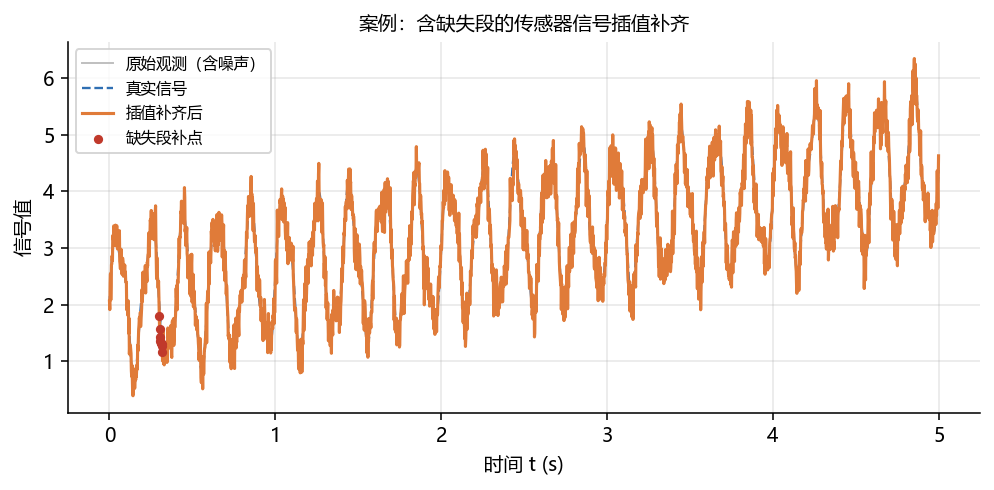
\includegraphics[keepaspectratio,alt={案例：含缺失段的信号插值补齐}]{figures/03-scipy/case_signal.png}}
\caption{案例：含缺失段的信号插值补齐}
\end{figure}

\subsection{用 FFT 找主频}\label{ux7528-fft-ux627eux4e3bux9891}

先做线性去趋势，消除漂移带来的低频泄漏，再取 \texttt{rfft}。

\begin{Shaded}
\begin{Highlighting}[]
\ImportTok{from}\NormalTok{ scipy.fft }\ImportTok{import}\NormalTok{ rfft, rfftfreq}
\NormalTok{coef }\OperatorTok{=}\NormalTok{ np.polyfit(t, y\_filled, }\DecValTok{1}\NormalTok{)}
\NormalTok{detrend }\OperatorTok{=}\NormalTok{ y\_filled }\OperatorTok{{-}}\NormalTok{ np.polyval(coef, t)}

\NormalTok{Y }\OperatorTok{=}\NormalTok{ rfft(detrend)}
\NormalTok{freqs }\OperatorTok{=}\NormalTok{ rfftfreq(N, }\DecValTok{1}\OperatorTok{/}\NormalTok{fs)}
\NormalTok{amps }\OperatorTok{=}\NormalTok{ np.}\BuiltInTok{abs}\NormalTok{(Y)}
\NormalTok{order }\OperatorTok{=}\NormalTok{ np.argsort(amps)[::}\OperatorTok{{-}}\DecValTok{1}\NormalTok{]}
\ControlFlowTok{for}\NormalTok{ k }\KeywordTok{in}\NormalTok{ order[:}\DecValTok{5}\NormalTok{]:}
    \BuiltInTok{print}\NormalTok{(}\SpecialStringTok{f"f=}\SpecialCharTok{\{}\NormalTok{freqs[k]}\SpecialCharTok{:.2f\}}\SpecialStringTok{ Hz  amp=}\SpecialCharTok{\{}\NormalTok{amps[k]}\SpecialCharTok{:.2f\}}\SpecialStringTok{"}\NormalTok{)}
\end{Highlighting}
\end{Shaded}

\begin{Shaded}
\begin{Highlighting}[]
\NormalTok{f=5.00 Hz  amp=1503.72}
\NormalTok{f=12.00 Hz  amp=371.19}
\NormalTok{f=0.20 Hz  amp=34.16}
\NormalTok{f=0.40 Hz  amp=30.74}
\NormalTok{f=19.60 Hz  amp=29.16}
\end{Highlighting}
\end{Shaded}

主峰在 5 Hz（次峰是 12
Hz）与建模时的真实频率完全一致；低频小峰来自去趋势后的残余。

\begin{figure}
\centering
\pandocbounded{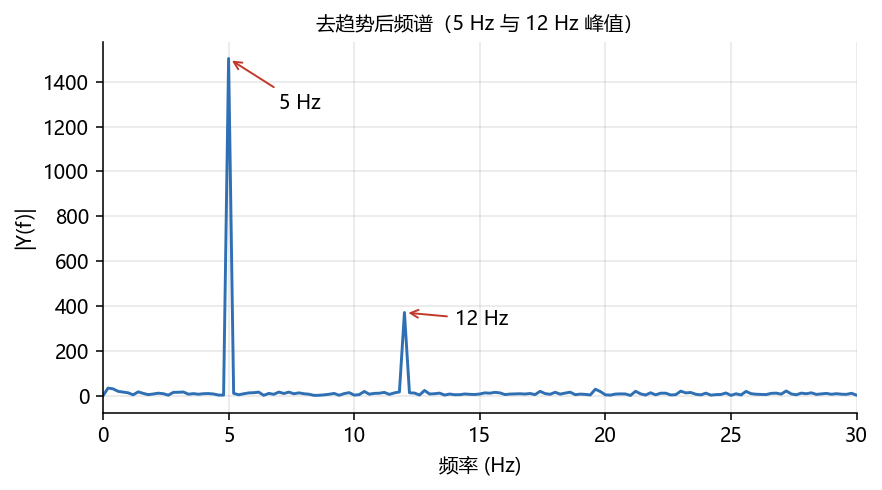
\includegraphics[keepaspectratio,alt={案例：去趋势后频谱}]{figures/03-scipy/case_fft.png}}
\caption{案例：去趋势后频谱}
\end{figure}

\subsection{\texorpdfstring{用 \texttt{curve\_fit}
拟合参数模型}{用 curve\_fit 拟合参数模型}}\label{ux7528-curve_fit-ux62dfux5408ux53c2ux6570ux6a21ux578b}

模型设为``常数 + 线性漂移 + 两个正弦''：

\[y(t)=c_1+c_2 t+A_1\sin(2\pi f_1 t+\varphi_1)+A_2\sin(2\pi f_2 t+\varphi_2)\]

\begin{Shaded}
\begin{Highlighting}[]
\ImportTok{from}\NormalTok{ scipy.optimize }\ImportTok{import}\NormalTok{ curve\_fit}

\KeywordTok{def}\NormalTok{ model(t, c1, c2, A1, f1, p1, A2, f2, p2):}
    \ControlFlowTok{return}\NormalTok{ c1 }\OperatorTok{+}\NormalTok{ c2}\OperatorTok{*}\NormalTok{t }\OperatorTok{+}\NormalTok{ A1}\OperatorTok{*}\NormalTok{np.sin(}\DecValTok{2}\OperatorTok{*}\NormalTok{np.pi}\OperatorTok{*}\NormalTok{f1}\OperatorTok{*}\NormalTok{t}\OperatorTok{+}\NormalTok{p1) }\OperatorTok{+}\NormalTok{ A2}\OperatorTok{*}\NormalTok{np.sin(}\DecValTok{2}\OperatorTok{*}\NormalTok{np.pi}\OperatorTok{*}\NormalTok{f2}\OperatorTok{*}\NormalTok{t}\OperatorTok{+}\NormalTok{p2)}

\NormalTok{popt, pcov }\OperatorTok{=}\NormalTok{ curve\_fit(model, t, y\_filled,}
\NormalTok{                       p0}\OperatorTok{=}\NormalTok{[}\DecValTok{2}\NormalTok{, }\FloatTok{0.5}\NormalTok{, }\FloatTok{1.2}\NormalTok{, }\DecValTok{5}\NormalTok{, }\DecValTok{0}\NormalTok{, }\FloatTok{0.3}\NormalTok{, }\DecValTok{12}\NormalTok{, }\DecValTok{0}\NormalTok{], maxfev}\OperatorTok{=}\DecValTok{50000}\NormalTok{)}
\NormalTok{perr }\OperatorTok{=}\NormalTok{ np.sqrt(np.diag(pcov))}
\BuiltInTok{print}\NormalTok{(}\StringTok{"拟合参数 ="}\NormalTok{, np.}\BuiltInTok{round}\NormalTok{(popt, }\DecValTok{4}\NormalTok{))}
\BuiltInTok{print}\NormalTok{(}\StringTok{"参数标准误 ="}\NormalTok{, np.}\BuiltInTok{round}\NormalTok{(perr, }\DecValTok{4}\NormalTok{))}
\NormalTok{resid }\OperatorTok{=}\NormalTok{ y\_filled }\OperatorTok{{-}}\NormalTok{ model(t, }\OperatorTok{*}\NormalTok{popt)}
\BuiltInTok{print}\NormalTok{(}\StringTok{"RMSE ="}\NormalTok{, }\BuiltInTok{round}\NormalTok{(}\BuiltInTok{float}\NormalTok{(np.sqrt(np.mean(resid}\OperatorTok{**}\DecValTok{2}\NormalTok{))), }\DecValTok{4}\NormalTok{))}
\BuiltInTok{print}\NormalTok{(}\StringTok{"f1 估计 ="}\NormalTok{, }\BuiltInTok{round}\NormalTok{(popt[}\DecValTok{3}\NormalTok{], }\DecValTok{3}\NormalTok{), }\StringTok{"   f2 估计 ="}\NormalTok{, }\BuiltInTok{round}\NormalTok{(popt[}\DecValTok{6}\NormalTok{], }\DecValTok{3}\NormalTok{))}
\end{Highlighting}
\end{Shaded}

\begin{Shaded}
\begin{Highlighting}[]
\NormalTok{拟合参数 = [ 1.9931  0.499   1.2042  5.0003 {-}0.0108  0.2977 12.0033 {-}0.064 ]}
\NormalTok{参数标准误 = [0.008  0.0028 0.0057 0.0005 0.0094 0.0057 0.0021 0.0382]}
\NormalTok{RMSE = 0.2009}
\NormalTok{f1 估计 = 5.0   f2 估计 = 12.003}
\end{Highlighting}
\end{Shaded}

拟合 \(f_1\approx5.00\) Hz、\(f_2\approx12.00\)
Hz，\(A_1\approx1.20\)、\(A_2\approx0.30\)，与真实模型高度一致；RMSE≈0.20
正是噪声标准差。

\begin{figure}
\centering
\pandocbounded{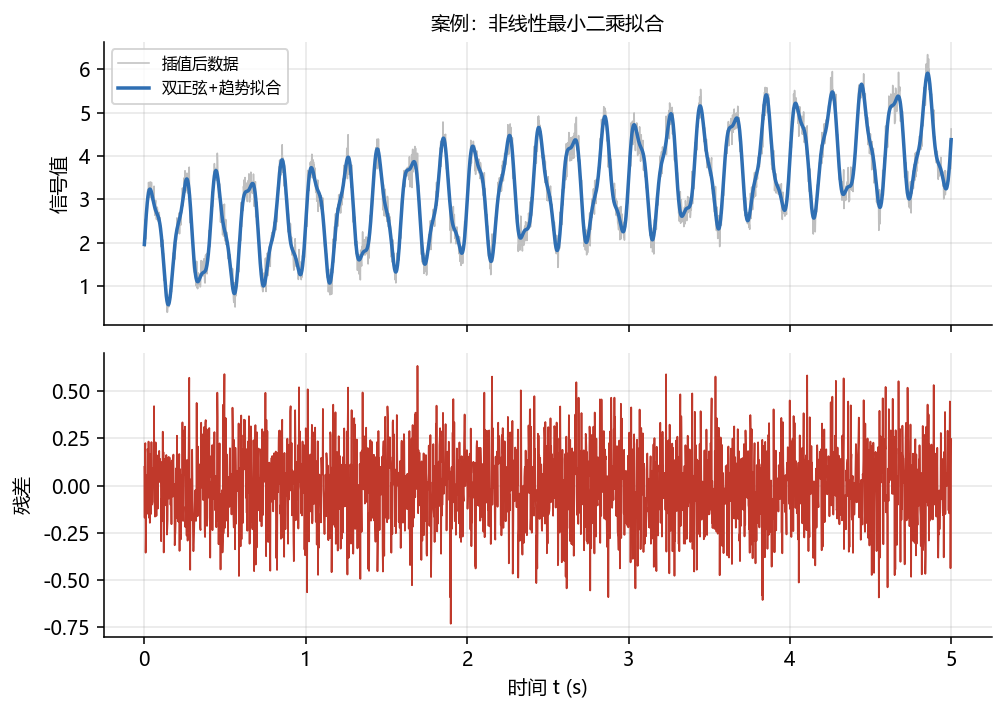
\includegraphics[keepaspectratio,alt={案例：拟合曲线与残差}]{figures/03-scipy/case_fit.png}}
\caption{案例：拟合曲线与残差}
\end{figure}

\subsection{\texorpdfstring{用 \texttt{trapezoid}
估计累积值}{用 trapezoid 估计累积值}}\label{ux7528-trapezoid-ux4f30ux8ba1ux7d2fux79efux503c}

\begin{Shaded}
\begin{Highlighting}[]
\ImportTok{from}\NormalTok{ scipy.integrate }\ImportTok{import}\NormalTok{ trapezoid}
\NormalTok{area }\OperatorTok{=}\NormalTok{ trapezoid(y\_filled, t)}
\BuiltInTok{print}\NormalTok{(}\StringTok{"5 秒内信号累积值 ="}\NormalTok{, }\BuiltInTok{round}\NormalTok{(}\BuiltInTok{float}\NormalTok{(area), }\DecValTok{4}\NormalTok{))}
\end{Highlighting}
\end{Shaded}

\begin{Shaded}
\begin{Highlighting}[]
\NormalTok{5 秒内信号累积值 = 16.1939}
\end{Highlighting}
\end{Shaded}

该值可理解为``总剂量/总能量''，是积分在工程中的一个典型用途。

\subsection{用 t
检验比较两段时间}\label{ux7528-t-ux68c0ux9a8cux6bd4ux8f83ux4e24ux6bb5ux65f6ux95f4}

线性漂移使后半段均值更高，用 \texttt{ttest\_ind} 验证。

\begin{Shaded}
\begin{Highlighting}[]
\ImportTok{from}\NormalTok{ scipy.stats }\ImportTok{import}\NormalTok{ ttest\_ind}
\NormalTok{g1 }\OperatorTok{=}\NormalTok{ y\_filled[(t }\OperatorTok{\textgreater{}=} \DecValTok{0}\NormalTok{) }\OperatorTok{\&}\NormalTok{ (t }\OperatorTok{\textless{}} \DecValTok{1}\NormalTok{)]}
\NormalTok{g2 }\OperatorTok{=}\NormalTok{ y\_filled[(t }\OperatorTok{\textgreater{}=} \DecValTok{4}\NormalTok{) }\OperatorTok{\&}\NormalTok{ (t }\OperatorTok{\textless{}} \DecValTok{5}\NormalTok{)]}
\NormalTok{res }\OperatorTok{=}\NormalTok{ ttest\_ind(g1, g2)}
\BuiltInTok{print}\NormalTok{(}\SpecialStringTok{f"前1s均值=}\SpecialCharTok{\{}\NormalTok{g1}\SpecialCharTok{.}\NormalTok{mean()}\SpecialCharTok{:.4f\}}\SpecialStringTok{, 后1s均值=}\SpecialCharTok{\{}\NormalTok{g2}\SpecialCharTok{.}\NormalTok{mean()}\SpecialCharTok{:.4f\}}\SpecialStringTok{"}\NormalTok{)}
\BuiltInTok{print}\NormalTok{(}\SpecialStringTok{f"t=}\SpecialCharTok{\{}\NormalTok{res}\SpecialCharTok{.}\NormalTok{statistic}\SpecialCharTok{:.3f\}}\SpecialStringTok{, p=}\SpecialCharTok{\{}\NormalTok{res}\SpecialCharTok{.}\NormalTok{pvalue}\SpecialCharTok{:.3e\}}\SpecialStringTok{"}\NormalTok{)}
\end{Highlighting}
\end{Shaded}

\begin{Shaded}
\begin{Highlighting}[]
\NormalTok{前1s均值=2.2442, 后1s均值=4.2493}
\NormalTok{t={-}35.601, p=7.475e{-}180}
\end{Highlighting}
\end{Shaded}

p
值极小，说明前、后两段均值差异在统计上高度显著------这正是题目设计的线性漂移所导致的。

\begin{figure}
\centering
\pandocbounded{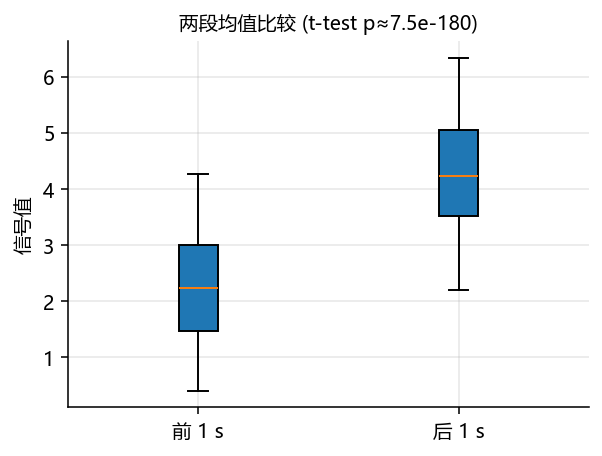
\includegraphics[keepaspectratio,alt={案例：两段时间均值比较}]{figures/03-scipy/case_stats.png}}
\caption{案例：两段时间均值比较}
\end{figure}

\subsection{小结}\label{ux5c0fux7ed3}

这个案例把本章五个工具包串成一条流水线：\textbf{插值补齐（03）→ FFT
定频（05）→ 非线性拟合（02）→ 积分（01）→ 假设检验（04）}。

{\def\LTcaptype{none} % do not increment counter
\begin{longtable}[]{@{}
  >{\raggedright\arraybackslash}p{(\linewidth - 4\tabcolsep) * \real{0.3333}}
  >{\raggedright\arraybackslash}p{(\linewidth - 4\tabcolsep) * \real{0.3333}}
  >{\raggedright\arraybackslash}p{(\linewidth - 4\tabcolsep) * \real{0.3333}}@{}}
\toprule\noalign{}
\begin{minipage}[b]{\linewidth}\raggedright
步骤
\end{minipage} & \begin{minipage}[b]{\linewidth}\raggedright
工具
\end{minipage} & \begin{minipage}[b]{\linewidth}\raggedright
产出
\end{minipage} \\
\midrule\noalign{}
\endhead
\bottomrule\noalign{}
\endlastfoot
补齐缺失 & \texttt{CubicSpline} & 完整时间序列 \\
频谱分析 & \texttt{rfft}/\texttt{rfftfreq} & 主频 5 Hz、12 Hz \\
参数化建模 & \texttt{curve\_fit} &
\(c_1,c_2,A_1,f_1,\varphi_1,A_2,f_2,\varphi_2\) \\
累积量 & \texttt{trapezoid} & 16.1939 \\
均值比较 & \texttt{ttest\_ind} & t=-35.60，p≈7.5e-180 \\
\end{longtable}
}

\subsection{拓展任务}\label{ux62d3ux5c55ux4efbux52a1-5}

\begin{enumerate}
\def\labelenumi{\arabic{enumi}.}
\tightlist
\item
  把缺失段加宽（如 0.30--0.50 s），观察插值误差如何变化；
\item
  用 \texttt{scipy.signal.butter} 低通（截止 10 Hz）滤除 12 Hz
  分量后重新拟合，比较残差；
\item
  把``前 1 s vs 后 1 s''换成``前 2.5 s vs 后 2.5 s''，看 p
  值变化并解释；
\item
  用 statsmodels 对三段时间做单因素 ANOVA + Tukey 事后比较。
\end{enumerate}

\subsection{延伸阅读}\label{ux5ef6ux4f38ux9605ux8bfb-15}

\begin{itemize}
\tightlist
\item
  SciPy 插值 / FFT / 优化官方文档见各节``官方文档/参考入口''。
\item
  信号处理完整示例：https://docs.scipy.org/doc/scipy/tutorial/fft.html
\item
  statsmodels 多重比较：https://www.statsmodels.org/stable/stats.html
\end{itemize}

\section{07
常见误区与技巧}\label{ux5e38ux89c1ux8befux533aux4e0eux6280ux5de7-2}

\begin{quote}
本章为新增``查漏补缺''页：把学生在 SciPy
上最容易踩的坑集中列出，并给出正确写法、性能与调试建议。
\end{quote}

\subsection{1.
高频误区速查表}\label{ux9ad8ux9891ux8befux533aux901fux67e5ux8868-2}

{\def\LTcaptype{none} % do not increment counter
\begin{longtable}[]{@{}
  >{\raggedright\arraybackslash}p{(\linewidth - 6\tabcolsep) * \real{0.2500}}
  >{\raggedright\arraybackslash}p{(\linewidth - 6\tabcolsep) * \real{0.2500}}
  >{\raggedright\arraybackslash}p{(\linewidth - 6\tabcolsep) * \real{0.2500}}
  >{\raggedright\arraybackslash}p{(\linewidth - 6\tabcolsep) * \real{0.2500}}@{}}
\toprule\noalign{}
\begin{minipage}[b]{\linewidth}\raggedright
\#
\end{minipage} & \begin{minipage}[b]{\linewidth}\raggedright
误区 / 错误写法
\end{minipage} & \begin{minipage}[b]{\linewidth}\raggedright
正确做法
\end{minipage} & \begin{minipage}[b]{\linewidth}\raggedright
原因
\end{minipage} \\
\midrule\noalign{}
\endhead
\bottomrule\noalign{}
\endlastfoot
1 & \texttt{from\ scipy.integrate\ import\ trapz} & 用
\texttt{trapezoid} & SciPy 1.15 已移除 \texttt{trapz} \\
2 & \texttt{odeint} 写 \texttt{func(t,\ y)} & 写成 \texttt{func(y,\ t)}
& \texttt{odeint} 的签名是 \texttt{(y,\ t)}，\texttt{solve\_ivp} 才是
\texttt{(t,\ y)} \\
3 & \texttt{solve\_ivp(f,\ 0,\ 5,\ y0)} &
\texttt{solve\_ivp(f,\ (0,5),\ y0)} & \texttt{t\_span} 是二元组 \\
4 & \texttt{quad(f,0,1)} 然后当数组用 &
\texttt{value,\ err\ =\ quad(...)} & \texttt{quad} 返回
\texttt{(value,\ error)} 元组 \\
5 & 用 \texttt{brent} 求根 & 求根用
\texttt{brentq}/\texttt{fsolve}/\texttt{root} & \texttt{brent}
求极小值，\texttt{brentq} 求根 \\
6 & \texttt{linprog(c)} 直接当最大化用 & 最大化时 \texttt{c} 取负 &
\texttt{linprog} 默认最小化 \\
7 & \texttt{linear\_sum\_assignment} 后直接 \texttt{cost.sum()} &
\texttt{cost{[}row\_ind,\ col\_ind{]}.sum()} &
返回索引配对，需用索引取成本 \\
8 & \texttt{minimize} 约束写成 \texttt{fun(x)\ \textless{}=\ 0} &
\texttt{ineq} 表示 \texttt{fun(x)\ \textgreater{}=\ 0} &
约束符号方向易反 \\
9 & 不给 \texttt{p0} 就 \texttt{curve\_fit} & 给接近真实值的初值 &
非线性最小二乘对初值敏感 \\
10 & 用 \texttt{interp2d} 做新代码 & 用
\texttt{RegularGridInterpolator}/\texttt{griddata} & \texttt{interp2d}
已废弃 \\
11 & 对噪声数据做样条插值 & 改为 \texttt{curve\_fit}/\texttt{np.polyfit}
& 插值会``穿过噪声'' \\
12 & \texttt{griddata} 在凸包外直接外推 & 自行判断并处理 \texttt{nan} &
\texttt{griddata} 不默认外推 \\
13 & \texttt{butter(Wn=cutoff)} & \texttt{Wn\ =\ cutoff\ /\ (fs/2)} &
\texttt{Wn} 是归一化频率 \\
14 & 把 \texttt{fft} 幅值当真实幅度 & 单边需乘 \(2/N\)；或用
\texttt{rfft} 后归一化 & \texttt{fft} 未除以 \(N\) \\
15 & 统计 p\textless0.05 就说``差异很大'' & 同时看效应量/置信区间 & p
值不度量重要性 \\
16 & 不做正态性检验就小样本 t 检验 & 小样本先 \texttt{shapiro} & t
检验假设近似正态 \\
17 & ANOVA 显著后不做事后比较 & 用 \texttt{pairwise\_tukeyhsd} &
需找具体差异组 \\
18 & 随机模拟不设种子 & \texttt{rng\ =\ np.random.default\_rng(seed)} &
便于复现与讨论 \\
\end{longtable}
}

\subsection{2.
原理级难点：版本迁移与新接口}\label{ux539fux7406ux7ea7ux96beux70b9ux7248ux672cux8fc1ux79fbux4e0eux65b0ux63a5ux53e3}

\begin{quote}
SciPy
迭代较快，老教材中的某些函数已改名或废弃。写新代码时以官方最新文档为准。
\end{quote}

{\def\LTcaptype{none} % do not increment counter
\begin{longtable}[]{@{}
  >{\raggedright\arraybackslash}p{(\linewidth - 4\tabcolsep) * \real{0.3333}}
  >{\raggedright\arraybackslash}p{(\linewidth - 4\tabcolsep) * \real{0.3333}}
  >{\raggedright\arraybackslash}p{(\linewidth - 4\tabcolsep) * \real{0.3333}}@{}}
\toprule\noalign{}
\begin{minipage}[b]{\linewidth}\raggedright
老写法
\end{minipage} & \begin{minipage}[b]{\linewidth}\raggedright
新写法
\end{minipage} & \begin{minipage}[b]{\linewidth}\raggedright
说明
\end{minipage} \\
\midrule\noalign{}
\endhead
\bottomrule\noalign{}
\endlastfoot
\texttt{scipy.integrate.trapz} & \texttt{scipy.integrate.trapezoid} &
同名函数改名 \\
\texttt{scipy.integrate.odeint}（仍可用） & 推荐 \texttt{solve\_ivp} &
新接口更灵活，支持事件/设置 \\
\texttt{scipy.optimize.leastsq}（仍可用） & 推荐 \texttt{curve\_fit} &
接口更友好，返回协方差 \\
\texttt{scipy.optimize.fmin}（仍可用） &
\texttt{minimize(method=\textquotesingle{}Nelder-Mead\textquotesingle{})}
& 统一入口 \\
\texttt{scipy.interpolate.interp2d} & \texttt{RegularGridInterpolator} &
\texttt{interp2d} 已废弃 \\
\texttt{scipy.fftpack} & \texttt{scipy.fft} & 新模块，接口更好 \\
\end{longtable}
}

\subsection{3. 性能技巧}\label{ux6027ux80fdux6280ux5de7-2}

\begin{itemize}
\tightlist
\item
  \textbf{向量化优先}：能用 NumPy 数组一次算完就不要 Python 循环；
\item
  \textbf{FFT 用
  \texttt{rfft}}：实数信号只用一半复数，速度与内存都省一半；
\item
  \textbf{插值选方法}：线性插值最快，三次样条更光滑但更慢；大数据散点可先
  \texttt{cKDTree} 再 \texttt{griddata}；
\item
  \textbf{\texttt{curve\_fit} 给 \texttt{maxfev}}：复杂模型设
  \texttt{maxfev=50000} 避免``达到最大调用次数''而失败；
\item
  \textbf{积分用 \texttt{quad}
  而非固定步长}：自适应能在光滑区间少算、在陡峭区间加密；
\item
  \textbf{优化设
  \texttt{bounds}/\texttt{constraints}}：有约束问题别用无约束方法，容易跑出物理合理区间；
\item
  \textbf{多进程并行}：\texttt{scipy.optimize.differential\_evolution}
  等全局方法天然可并行，用 \texttt{workers} 参数。
\end{itemize}

\subsection{4. 调试建议}\label{ux8c03ux8bd5ux5efaux8bae-2}

\begin{enumerate}
\def\labelenumi{\arabic{enumi}.}
\tightlist
\item
  \textbf{打印形状/版本}：\texttt{print(x.shape,\ scipy.\_\_version\_\_)}，先确认输入维度正确；
\item
  \textbf{检查收敛标志}：\texttt{root}、\texttt{minimize}、\texttt{curve\_fit}
  都看 \texttt{success}/\texttt{message}，别只看结果；
\item
  \textbf{给初值/区间}：\texttt{curve\_fit} 用
  \texttt{p0}；\texttt{brentq} 用 \texttt{brack}；\texttt{minimize}
  用多组初值；
\item
  \textbf{固定随机种子}：\texttt{default\_rng(seed)}，保证课堂演示与作业可复现；
\item
  \textbf{异常值/NaN}：先用 \texttt{np.isnan}/\texttt{np.isinf}
  检查数据，再做插值/拟合；
\item
  \textbf{用图直观检查}：把数据、插值曲线、拟合曲线、频谱画出来，问题一眼可见；
\item
  \textbf{测试小数据}：先用 5
  个点验证函数是否返回合理，再放大到真实数据。
\end{enumerate}

\subsection{5. 自测清单}\label{ux81eaux6d4bux6e05ux5355}

\begin{itemize}
\tightlist
\item[$\square$]
  能用 \texttt{quad}/\texttt{dblquad}/\texttt{trapezoid} 求定积分；
\item[$\square$]
  能把二阶 ODE 化成一阶方程组并用 \texttt{odeint}/\texttt{solve\_ivp}
  求解；
\item[$\square$]
  能用 \texttt{brentq} 求根、\texttt{brent} 求极小值，并说清区别；
\item[$\square$]
  能用
  \texttt{minimize}/\texttt{linprog}/\texttt{linear\_sum\_assignment}
  解决无约束/线性规划/指派问题；
\item[$\square$]
  能用 \texttt{curve\_fit} 拟合参数并读取 \texttt{pcov}；
\item[$\square$]
  能用
  \texttt{CubicSpline}/\texttt{RegularGridInterpolator}/\texttt{griddata}
  完成一维/二维/散点插值；
\item[$\square$]
  能说出插值 vs 拟合的区别；
\item[$\square$]
  能用
  \texttt{shapiro}/\texttt{ttest\_ind}/\texttt{ttest\_rel}/\texttt{chi2\_contingency}/\texttt{f\_oneway}
  完成检验并解读 p 值；
\item[$\square$]
  能用 \texttt{rfft}/\texttt{rfftfreq} 找主频，用
  \texttt{butter}+\texttt{lfilter} 做滤波；
\item[$\square$]
  能独立完成 06 综合案例并解释每一步。
\end{itemize}

\subsection{延伸阅读}\label{ux5ef6ux4f38ux9605ux8bfb-16}

\begin{itemize}
\tightlist
\item
  SciPy 官方``Release
  notes''查看版本变更：https://docs.scipy.org/doc/scipy/release.html
\item
  SciPy 性能 / 高阶技巧：https://scipy-lectures.org/
\item
  SciPy
  Cookbook（老但仍有参考价值）：https://scipy.github.io/old-wiki/pages/Cookbook/
\end{itemize}

\newpage
